\documentclass{beamer}
\usepackage[latin1]{inputenc,colortbl}
\usepackage{epsfig}
\usepackage{epstopdf}

%%%%%%%
\usepackage{color}
\definecolor{light-gray}{gray}{0.70}

%%%%%%% Animation Packages
\usepackage{tikz}
\usepackage{animate}



\usetheme{Frankfurt}
\setbeamertemplate{navigation symbols}{}
\setbeamertemplate{footline}[page number]
%\newtheorem{definition}{Definition}
\title[Dynamic Formation and Strategic Management of Web Services Communities]{Dynamic Formation and Strategic Management of Web Services Communities}
\author{Ehsan Khosrowshahi Asl\\ \vspace{0.2cm} Supervised by: \\Dr. Jamal Bentahar \\Dr. Hadi Otrok}
\institute{Department of Computer Science and Software Engineering\\Concordia University}
\date{September 1, 2015}
\begin{document}
%%%%%%%%%%%%%%%%%%%%%%%%%%%%%%%% frame1 title page %%%%%%%%%%%%%%%%%%%%%%%%%%%%%%%%%%%%%%%
%%%%%%%%%%%%%%%%%%%%%%%%%%%%%%%%%%%%%%%%%%%%%%%%%%%%%%%%%%%%%%%%%%%%%%%%%%%%%%
\begin{frame}
\titlepage
\end{frame}
%%%%%%%%%%%%%%%%%%%%%%%%%%%%%%%% frame2 outline page %%%%%%%%%%%%%%%%%%%%%%%%%%%%%%%%%%%%%
%%%%%%%%%%%%%%%%%%%%%%%%%%%%%%%%%%%%%%%%%%%%%%%%%%%%%%%%%%%%%%%%%%%%%%%%%%%%%%

\begin{frame}{Presentation Outline}
    \begin{itemize}
     	\itemsep=.5cm
    	\item {\bf Introduction}
    	\item Background and Literature Review
    	\item Proposed Research
    	\item Conclusion and Feature Work
    \end{itemize}
    % Amazon Web Services is a $5 billion business, and it’s growing 50% a year
    % AMAZON WEB SERVICES (AWS) CLOUD IS A $5 BILLION BUSINESS AND GROWING FAST
\end{frame}


%\begin{frame}
%\begin{tikzpicture}
%\node at (7.5,4) {A};
%    \uncover<2->{\draw [-, draw=black!70, line width=1] (8,4) -- +(1,0) coordinate (v4) {} ;}
%    \uncover<3->{\draw [-, draw=black!70, line width=1] (v4) -- +(0,-2) coordinate (v5) {} ;}
%    \uncover<4->{\draw [->, draw=black!70, line width=1] (v5) -- +(-1,0) ;}
%\uncover<5->{ \node at (7.5,2) {B};}
%\end{tikzpicture}
%\end{frame}

%\begin{frame}
%
%    \begin{figure}
%        \includegraphics<1>[width=1.0 \columnwidth]{figures/wsinternet.png}
%        \includegraphics<2>[width=1.0 \columnwidth]{figures/wscommunity2.png}
%        \caption{\only<1>{First Image}\only<2>{Second Image}}
%    \end{figure}
%
%\end{frame}



%%%%%%%%%%%%%%%%%%%%%%%%%%%%%%%% frame3 introduction %%%%%%%%%%%%%%%%%%%%%%%%%%%%%%%%%%%%%
%%%%%%%%%%%%%%%%%%%%%%%%%%%%%%%%%%%%%%%%%%%%%%%%%%%%%%%%%%%%%%%%%%%%%%%%%%%%%%
\section{Introduction}
%\section{Motivation}
\subsection{Motivation}


%%%%%%%%%%%%%%%%%%%%%%%%%%%%%%%%%%%%%%%%%%%%%%%%%%%%%%%%%%%%%%%%%%%%%%%%%%%%%%
\begin{frame}{Motivation}
    \begin{figure}[htbp]
        \centering
        %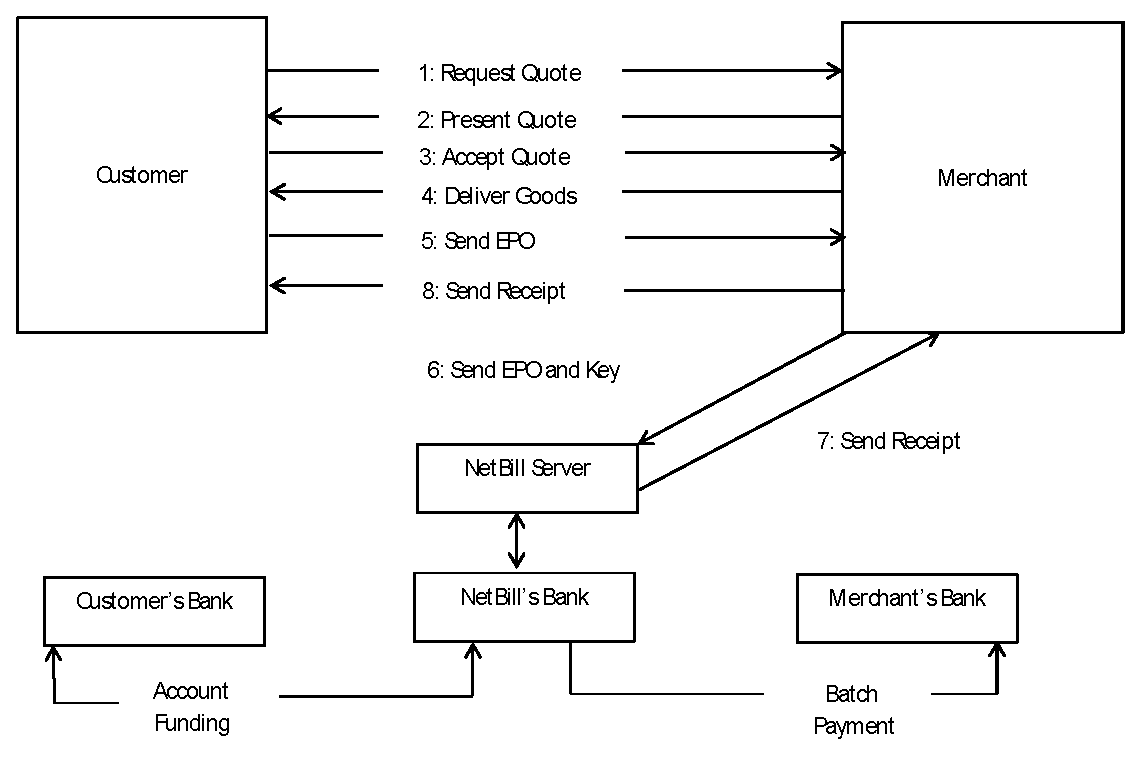
\includegraphics[width=12cm, height=8cm]{figures/figure1.eps}
        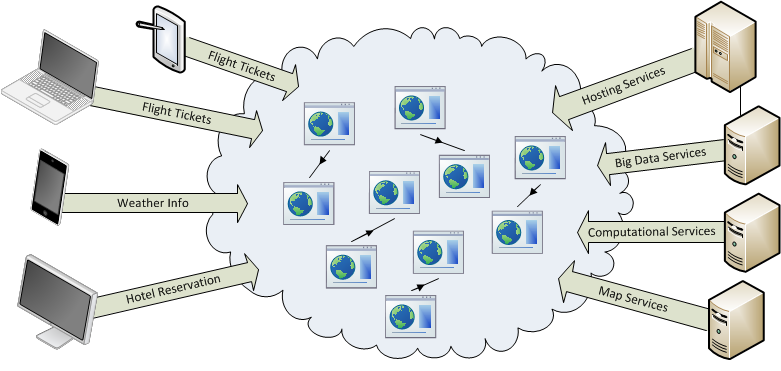
\includegraphics[width=0.9 \columnwidth]{figures/webservice_intro.png}
        %%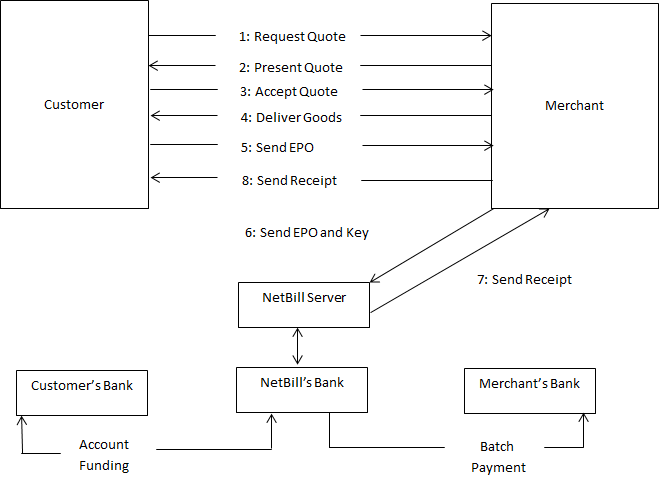
\includegraphics[scale=0.5]{figure1}
        %\caption{The NetBill payment protocol} \label{figure7}
    \end{figure}
    \begin{itemize}
        \item High reliance on web services created high competition and great business opportunities for online service developers
        \item \emph{\color{blue}Amazon Q1 2015 financial report:} Amazon Web Services is a \$5 billion business, and its growing 50\% a year
    \end{itemize}
\end{frame}

%%%%%%%%%%%%%%%%%%%%%%%%%%%%%%%%%%%%%%%%%%%%%%%%%%%%%%%%%%%%%%%%%%%%%%%%%%%%%%
\begin{frame}{Motivation}
    \begin{figure}[htbp]
        \centering
        %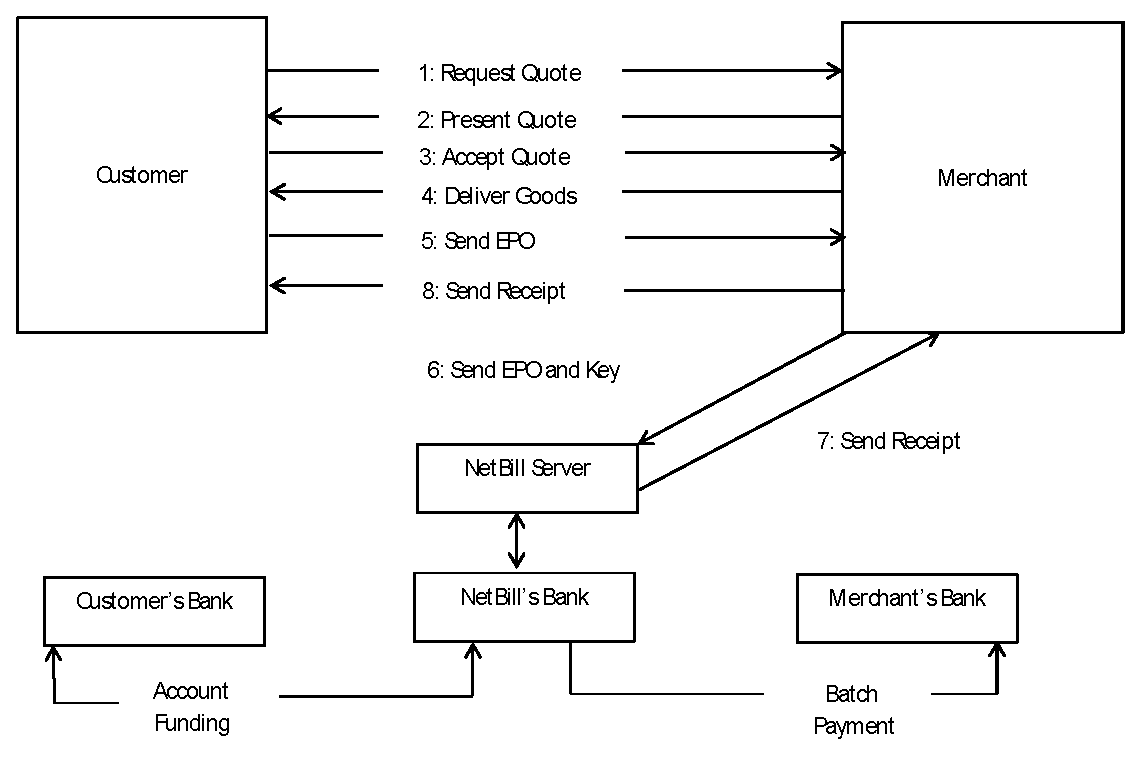
\includegraphics[width=12cm, height=8cm]{figures/figure1.eps}
        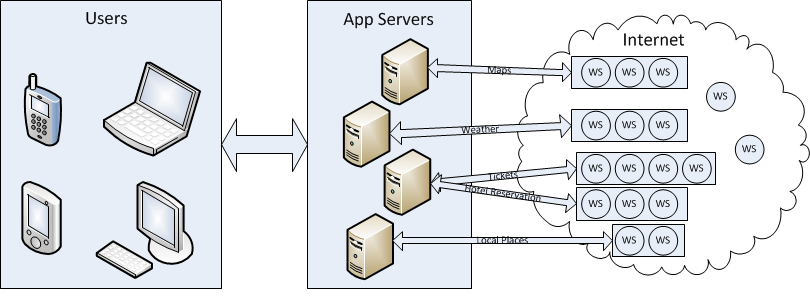
\includegraphics[width=1.0 \columnwidth]{figures/wsinternet.png}
        %%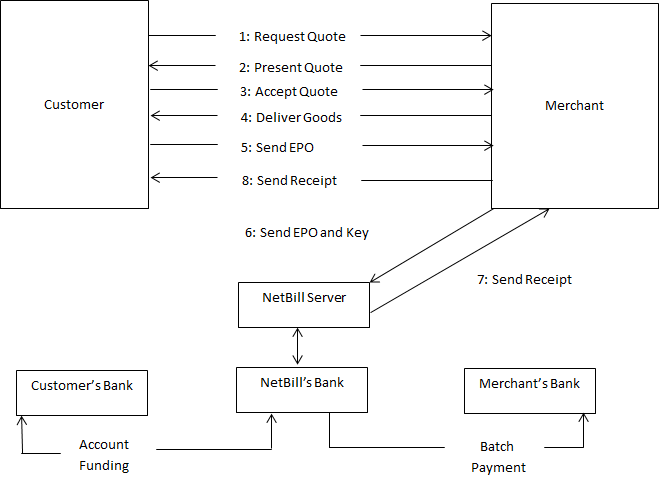
\includegraphics[scale=0.5]{figure1}
        %\caption{The NetBill payment protocol} \label{figure7}
    \end{figure}

    \begin{itemize}
        \item Community of web services: Clustering similar web services in order to:
        \begin{itemize}
            \item \textbf{Provide Better User Satisfaction Through High Availability and Responsiveness}.
            \item \textbf{Facilitate Web Service Discovery over Internet}.
            \item \textbf{Maintain high reputation and market share}.
        \end{itemize}
    \end{itemize}
\end{frame}

%%%%%%%%%%%%%%%%%%%%%%%%%%%%%%%%%%%%%%%%%%%%%%%%%%%%%%%%%%%%%%%%%%%%%%%%%%%%%%
%\subsection{Social commitments in MASs}
\begin{frame}{Communities of Web Services}

    \begin{figure}[htbp]
        \centering
        %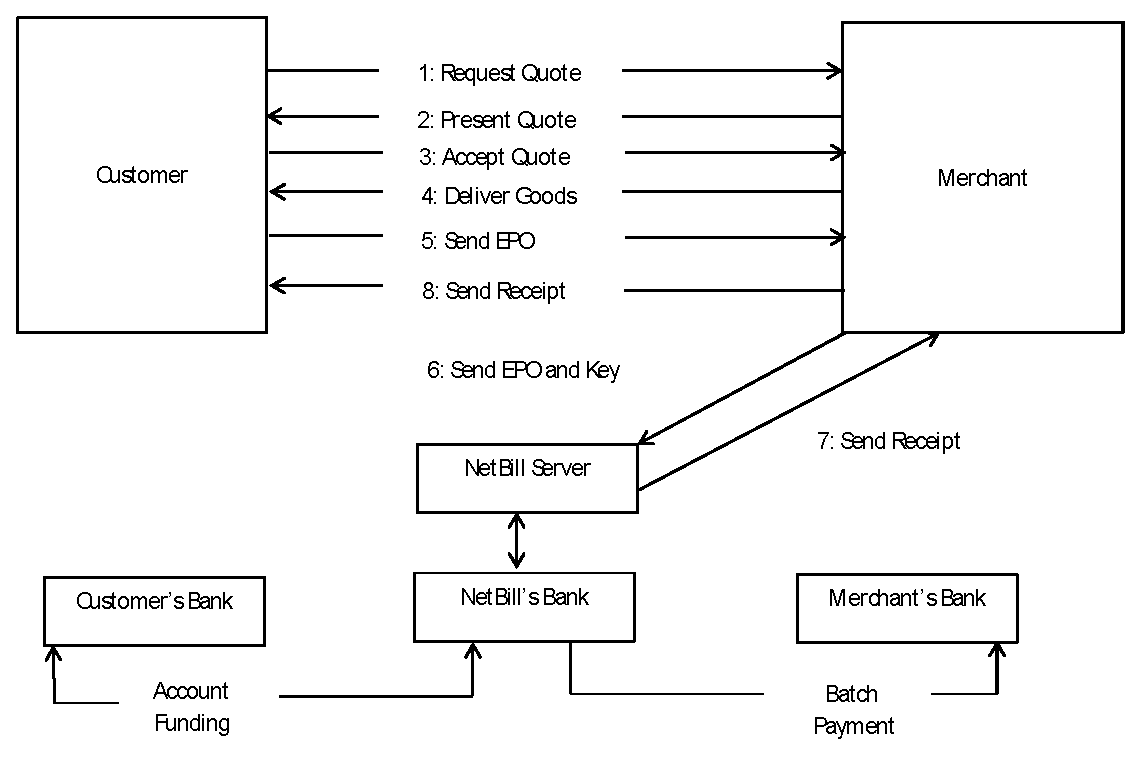
\includegraphics[width=12cm, height=8cm]{figures/figure1.eps}
        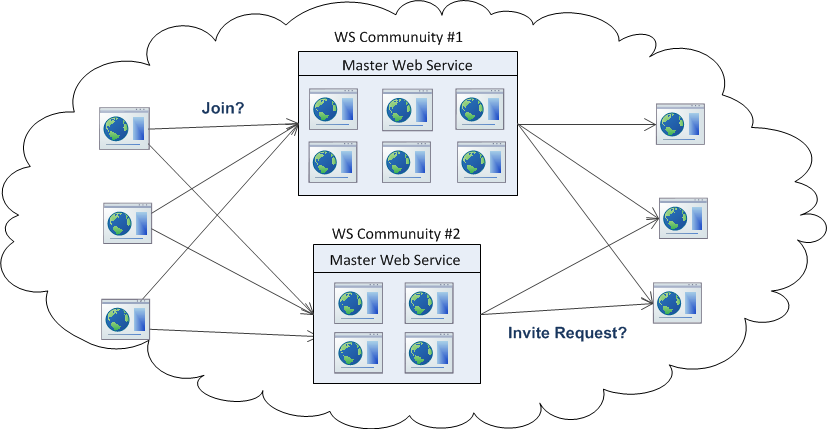
\includegraphics[width=0.85 \columnwidth]{figures/community_tasks.png}
        %%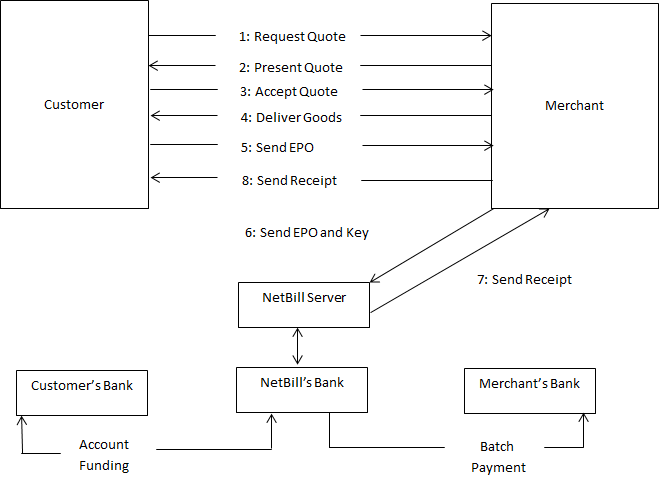
\includegraphics[scale=0.5]{figure1}
        %\caption{The NetBill payment protocol} \label{figure7}
    \end{figure}

    \begin{itemize}
        \itemsep=.35cm
    	\item \textbf{Communities of web services operations}
        \begin{itemize}
          \item Community development
          \item Web services attraction and retention
          \item Web service selection
        \end{itemize}                      	      	
    \end{itemize}
\end{frame}


%%%%%%%%%%%%%%%%%%%%%%%%%%%%%%%%%%%%%%%%%%%%%%%%%%%%%%%%%%%%%%%%%%%%%%%%%%%%%%
\begin{frame}{Problems and Research Questions}
%    \begin{figure}[htbp]
%        \centering
%        %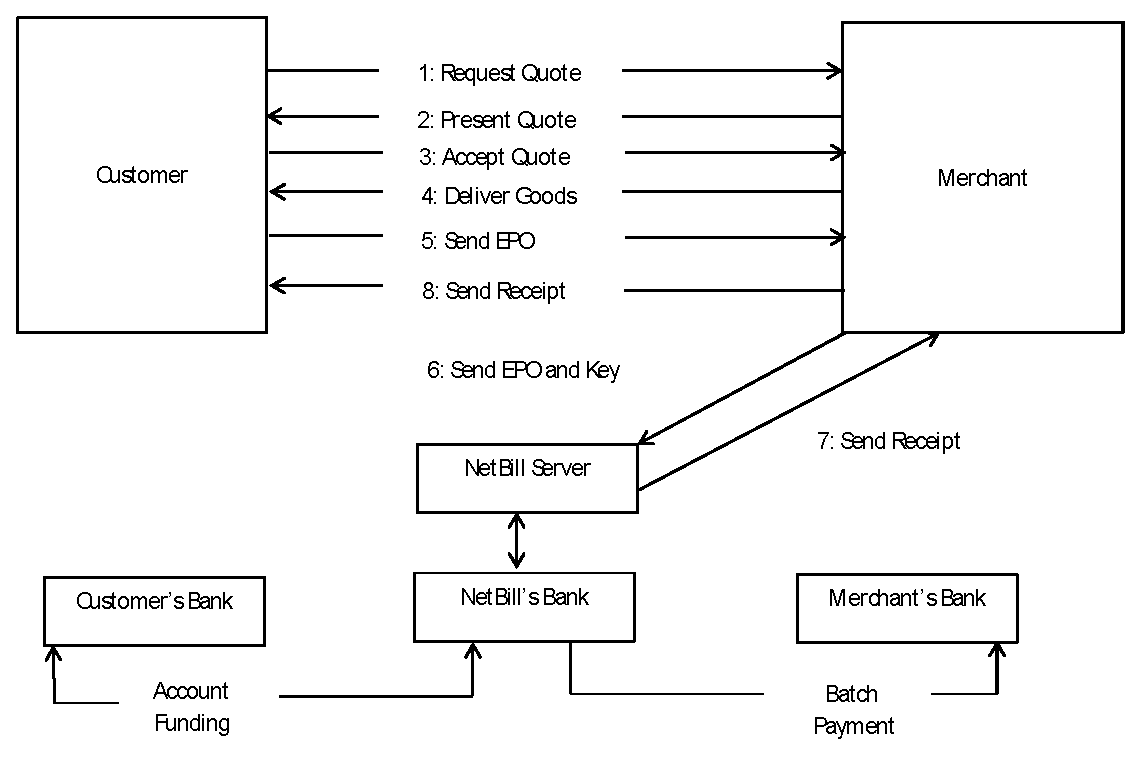
\includegraphics[width=12cm, height=8cm]{figures/figure1.eps}
%        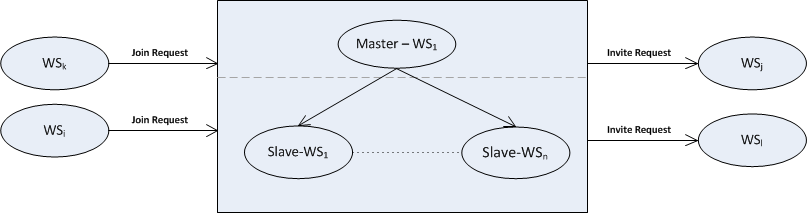
\includegraphics[width=0.6 \columnwidth]{figures/rq1.png}
%        %%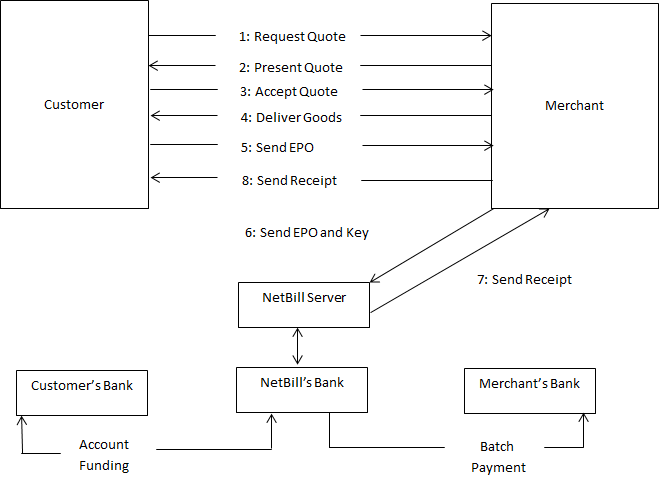
\includegraphics[scale=0.5]{figure1}
%        %\caption{The NetBill payment protocol} \label{figure7}
%    \end{figure}

    %\begin{itemize}
%        \item {\color{blue} Problem:} Community formation and membership management
%        \item {\color{blue} Methodology:} Cooperative Game Theory methods; covers fairness, stability and gain distribution
%    \end{itemize}

    \footnotesize{\colorbox{blue}{\color{white}{R1}} How can we model the community of agent-based services in order to maximize the utility
        of involved users, web services and community organizers?}\\
        \begin{itemize}
            \item Most of the work on communities of
            services are either user-centric and focus on user satisfaction
            or system-centric and focus on the whole system throughput, performance and utilization.
        \end{itemize}
    \vspace{0.3cm} \colorbox{blue}{\color{white}{R2}} How can we model fair and stable communities as coalitions of agent-based web services?\\
        \begin{itemize}
            \item All parties involved are self-interest agents and have the right to leave the community if they can improve their income in some other ways.
        \end{itemize}
    \vspace{0.3cm} \colorbox{blue}{\color{white}{R3}} How can we model and analyze the cooperation
        among the community members in realistic, applicable and practical settings?\\
        \begin{itemize}
            \item The first issue is about the performance evaluation of web services that are working together inside communities.
            \item The second issue is about the complexity of cooperative game theory solution concepts.
        \end{itemize}
\end{frame}

%%%%%%%%%%%%%%%%%%%%%%%%%%%%%%%%%%%%%%%%%%%%%%%%%%%%%%%%%%%%%%%%%%%%%%%%%%%%%%
\begin{frame}{Problems and Research Questions}
    \begin{figure}[htbp]
        \centering
        %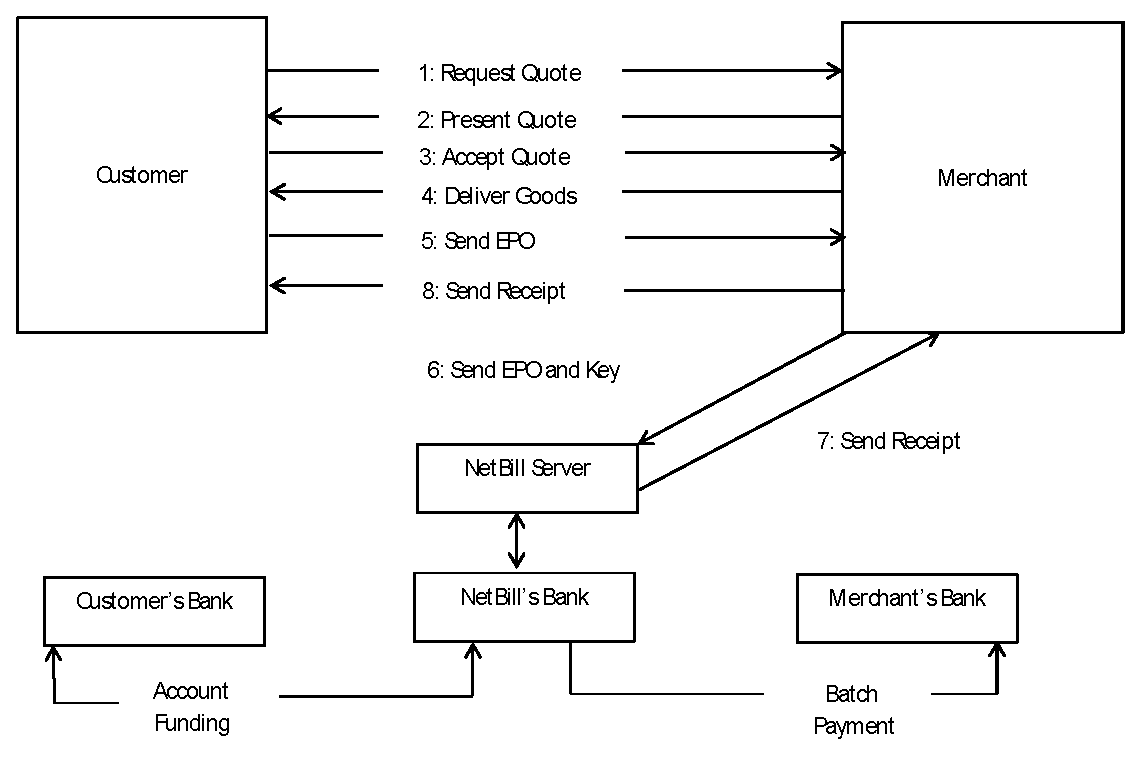
\includegraphics[width=12cm, height=8cm]{figures/figure1.eps}
        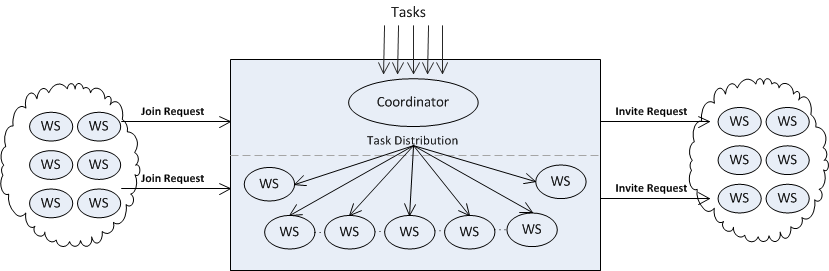
\includegraphics[width=1.0 \columnwidth]{figures/rq2.png}
        %%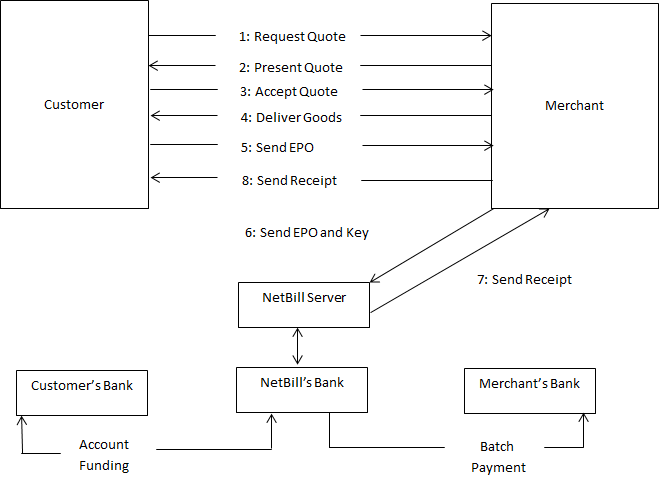
\includegraphics[scale=0.5]{figure1}
        %\caption{The NetBill payment protocol} \label{figure7}
    \end{figure}
    
    \footnotesize{\colorbox{blue}{\color{white}{R4}} How can we model a distributed decision making process for the problem of forming communities of services?}\\
        \begin{itemize}
            \item Centralized community structure has practical limitations among service providers            
        \end{itemize}
    \vspace{0.3cm} \colorbox{blue}{\color{white}{R5}} How can we train web services based on limited information to operate efficiently?\\
        \begin{itemize}
            \item Assumption of complete information is not practical in real world settings.
        \end{itemize}
\end{frame}

%%%%%%%%%%%%%%%%%%%%%%%%%%%%%%%%%%%%%%%%%%%%%%%%%%%%%%%%%%%%%%%%%%%%%%%%%%%%%%
\begin{frame}{Problems and Research Questions}
    \begin{figure}[h]
        \centering
         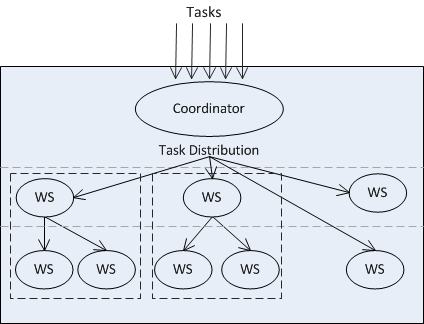
\includegraphics[scale=0.5]{figures/rq3.png}
%        \caption{Services are partitioned into competitive and cooperative
%        sets. Competitive services may get tasks directly from the master
%        agent and they can share it with other cooperative services in
%        their collaborative networks within the same community.}
        \label{architectureFigure}
    \end{figure}

    \footnotesize{\colorbox{blue}{\color{white}{R6}} How can we design a community model where both competitive and cooperative behaviors exist?}\\
        \begin{itemize}
            \item There is competitive environment \emph{inside communities} as well as cooperative behavior of communities.
        \end{itemize}
            
\end{frame}

%%%%%%%%%%%%%%%%%%%%%%%%%%%%%%%%%%%%%%%%%%%%%%%%%%%%%%%%%%%%%%%%%%%%%%%%%%%%%%%
\begin{frame}{Research Methodology}
    \begin{figure}[htbp]
        \centering
        %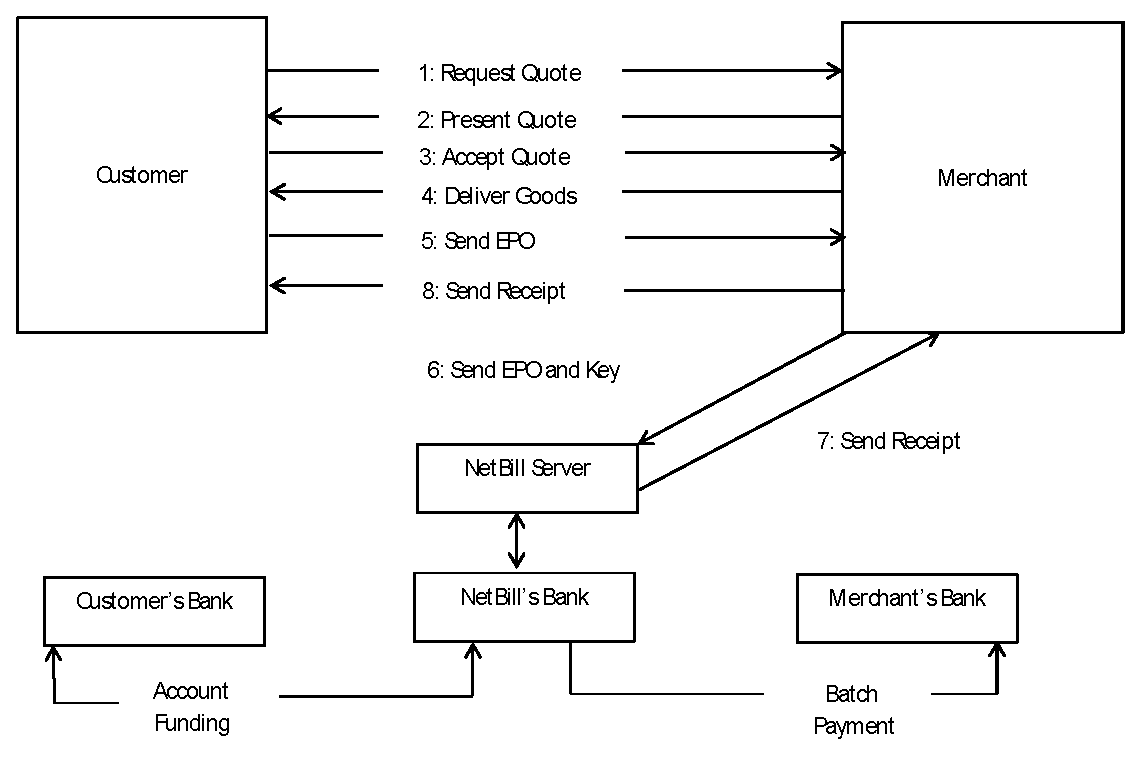
\includegraphics[width=12cm, height=8cm]{figures/figure1.eps}
        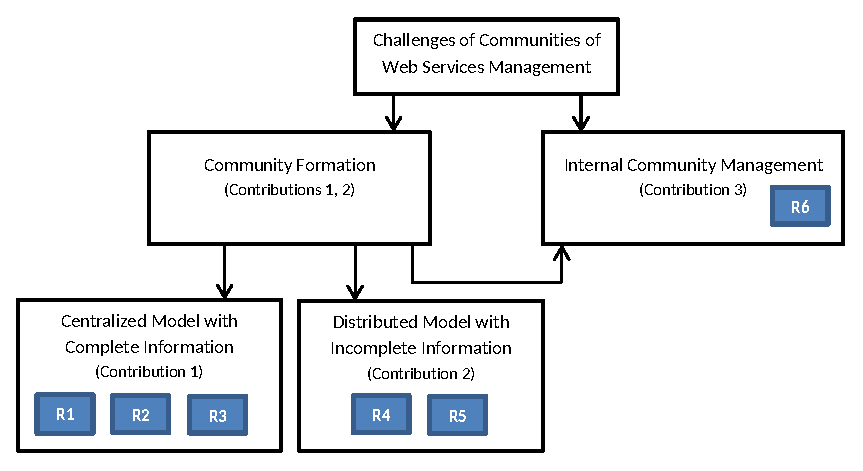
\includegraphics[width=0.9 \columnwidth]{figures/model.eps}
        %%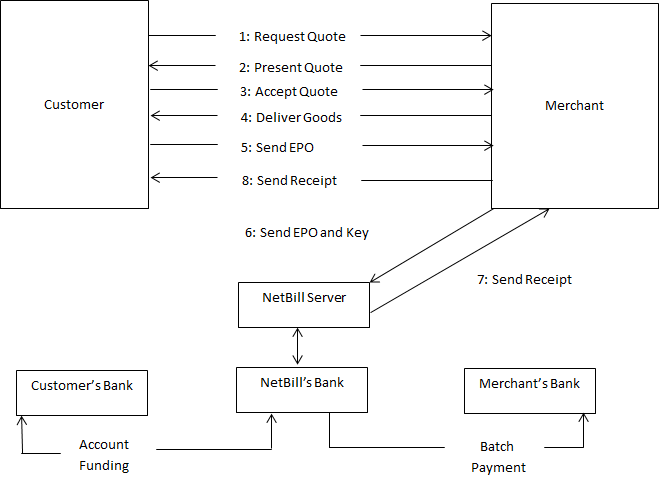
\includegraphics[scale=0.5]{figure1}
        %\caption{The NetBill payment protocol} \label{figure7}
    \end{figure}
\end{frame}


%%%%%%%%%%%%%%%%%%%%%%%%%%%%%%%%%%%%%%%%%%%%%%%%%%%%%%%%%%%%%%%%%%%%%%%%%%%%%%

%\subsection{Communities of Web Services}
%    \begin{frame}{Community of Web Services}
%       Communities of Web Services
%       \begin{itemize}
%           \item Ease and improve the process of Web services discovery in an open environment like the Internet
%       	\item Improve service quality, availability and responsiveness
%           \item Maintaining high reputation and market share
%       \end{itemize}

%       \begin{figure}[htbp]
%           \centering
            %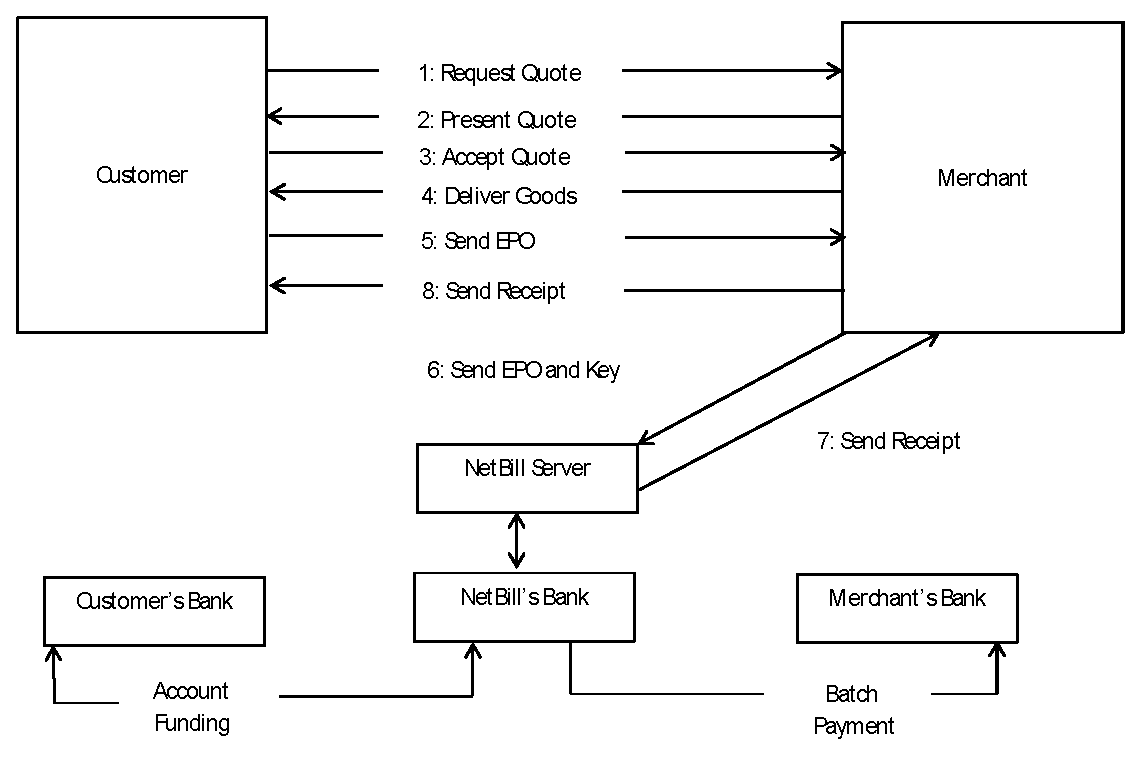
\includegraphics[width=12cm, height=8cm]{figures/figure1.eps}
%           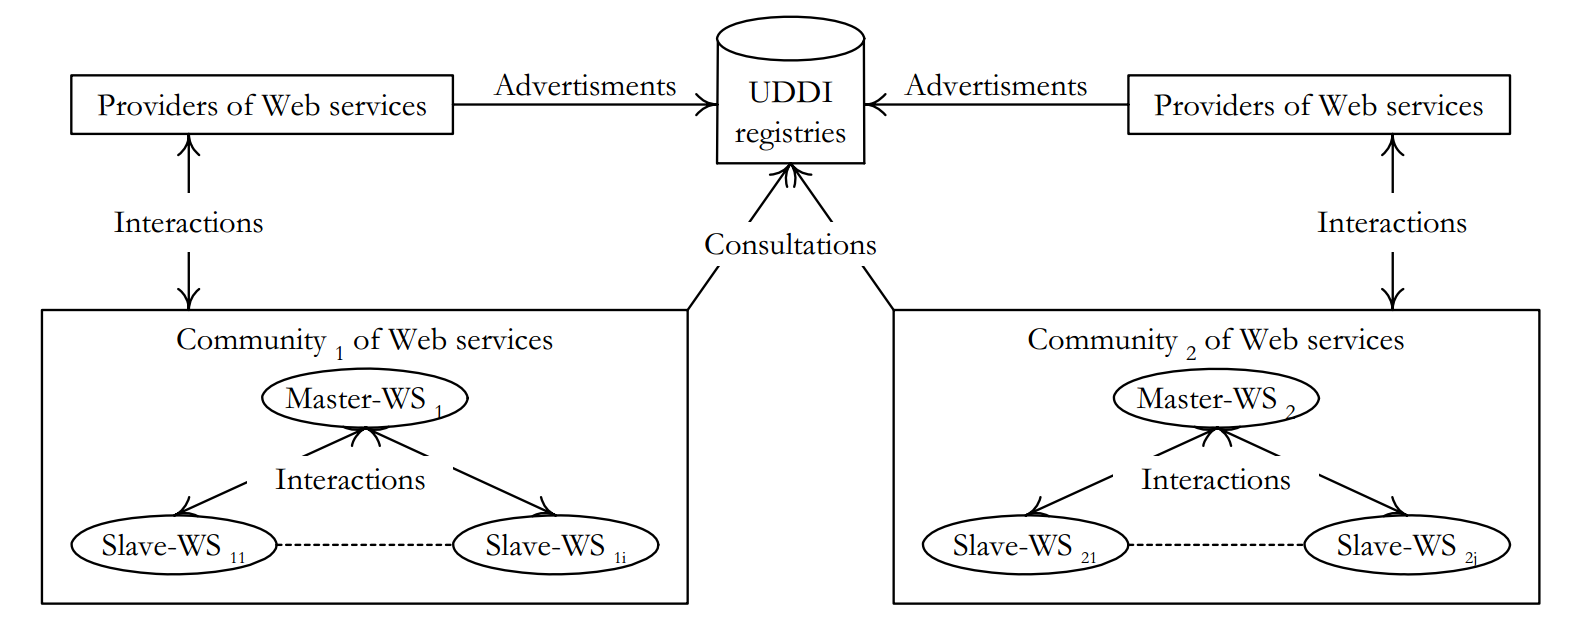
\includegraphics[width=1.0 \columnwidth]{figures/wscommunity2.png}
            %%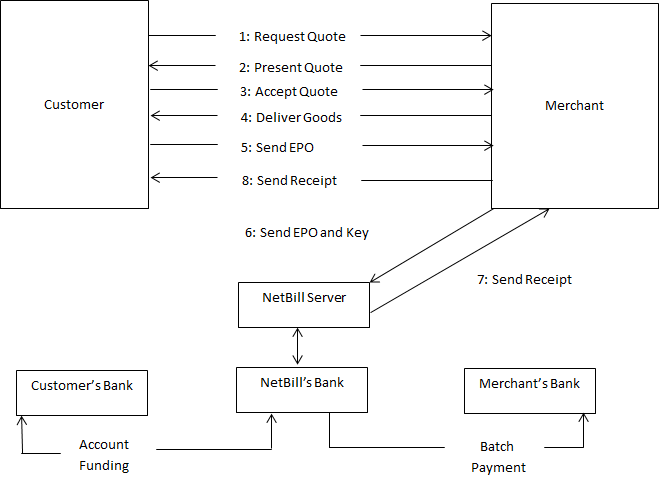
\includegraphics[scale=0.5]{figure1}
            %\caption{The NetBill payment protocol} \label{figure7}
%       \end{figure}

%   \end{frame}
%%%%%%%%%%%%%%%%%%%%%%%%%%%%%%%% frame10 Background and Literature Review %%%%%%%%%%%%%%%%%%%%%%%%%%%%%%%%%%%%%




%\begin{frame}{Problems and Research Questions}
%
%\begin{itemize}
%    \item \textbf{How can we model the
%        community of agent-based services in order to maximize the utility
%        of involved users, web services and community organizers?}
%        \begin{itemize}
%            \item Most of the work on communities of
%            services are either user-centric and focus on user satisfaction
%            or system-centric and focus on the whole system throughput, performance and utilization.
%        \end{itemize}
%
%
%    \item \textbf{How can we model fair and stable communities as coalitions
%        of agent-based web services?}
%        \begin{itemize}
%            \item All parties involved are self-interest agents and have the right to leave the community if they can improve their income in some other ways.
%        \end{itemize}
%
%\end{itemize}
%
%\end{frame}
%%%%%%%%%%%%%%%%%%%%%%%%%%%%%%%%%%%%%%%%%%%%%%%%%%%%%%%%%%%%%%%%%%%%%%%%%%%%%%%
%
%
%\begin{frame}{Continue: Problems and Research Questions}
% \begin{itemize}
%   \item \textbf{How can we model and analyze the cooperation
%        among the community members in realistic, applicable and practical
%        settings?}
%        \begin{itemize}
%            \item The first issue is about the evaluation of web services that are working together inside communities.
%            \item The second issue is about the complexity of cooperative game theory solution concepts.
%        \end{itemize}
%
%   \item \textbf{Considering competitive environment with communities how can services choose best strategy within communities?}
%        \begin{itemize}
%            \item Services can learn over time how and when to compete for tasks according to their and others capabilities.
%        \end{itemize}
%\end{itemize}
%\end{frame}
%
%%%%%%%%%%%%%%%%%%%%%%%%%%%%%%%%%%%%%%%%%%%%%%%%%%%%%%%%%%%%%%%%%%%%%%%%%%%%%%%
%\begin{frame}{Continue: Problems and Research Questions}
% \begin{itemize}
%   \item \textbf{How can we model a distributed decision making process for the problem of forming communities of services?}
%        \begin{itemize}
%            \item In real world scenarios, decisions made by independent service providers are highly distributed.
%            \item Agents can get trained so they can operate efficiently when information is incomplete
%        \end{itemize}
%
%   \item \textbf{Considering competitive environment with communities how can services choose best strategy within communities?}
%        \begin{itemize}
%            \item Services can learn over time how and when to compete for tasks according to their and others capabilities.
%        \end{itemize}
%\end{itemize}
%\end{frame}
%%%%%%%%%%%%%%%%%%%%%%%%%%%%%%%%%%%%%%%%%%%%%%%%%%%%%%%%%%%%%%%%%%%%%%%%%%%%%%%
%%%%%%%%%%%%%%%%%%%%%%%%%%%%%%%%%%%%%%%%%%%%%%%%%%%%%%%%%%%%%%%%%%%%%%%%%%%%%%%
%    \begin{frame}{Multi-Agent Systems MASs}
%        \begin{itemize}
%            \itemsep=.35cm
%        	\item Multi-Agent System (MAS).
%            %\item Autonomous agents.
%        	\item Knowledge in MASs.
%            \item Social commitments in MASs.
%        \end{itemize}
%\end{frame}

%%%%%%%%%%%%%%%%%%%%%%%%%%%%%%%%%%%%%%%%%%%%%%%%%%%%%%%%%%%%%%%%%%%%%%%%%%%%%%
\section{Background}
\begin{frame}{Presentation Outline}
    \begin{itemize}
     	\itemsep=.5cm
    	\item Introduction
    	\item {\bf Background and Literature Review}
    	\item Proposed Research
    	\item Conclusion and Feature Work
    \end{itemize}
\end{frame}

%%%%%%%%%%%%%%%%%%%%%%%%%%%%%%%% frame9 Background and Literature Review %%%%%%%%%%%%%%%%%%%%%%%%%%%%%%%%%%%%%
%%%%%%%%%%%%%%%%%%%%%%%%%%%%%%%%%%%%%%%%%%%%%%%%%%%%%%%%%%%%%%%%%%%%%%%%%%%%%%

%%%%%%%%%%%%%%%%%%%%%%%%%%%%%%%%%%%%%%%%%%%%%%%%%%%%%%%%%%%%%%%%%%%%%%%%%%%%%%
%\subsection{Social commitments in MASs}
\begin{frame}{Communities of Web Services}
    \begin{figure}[htbp]
        \centering
        %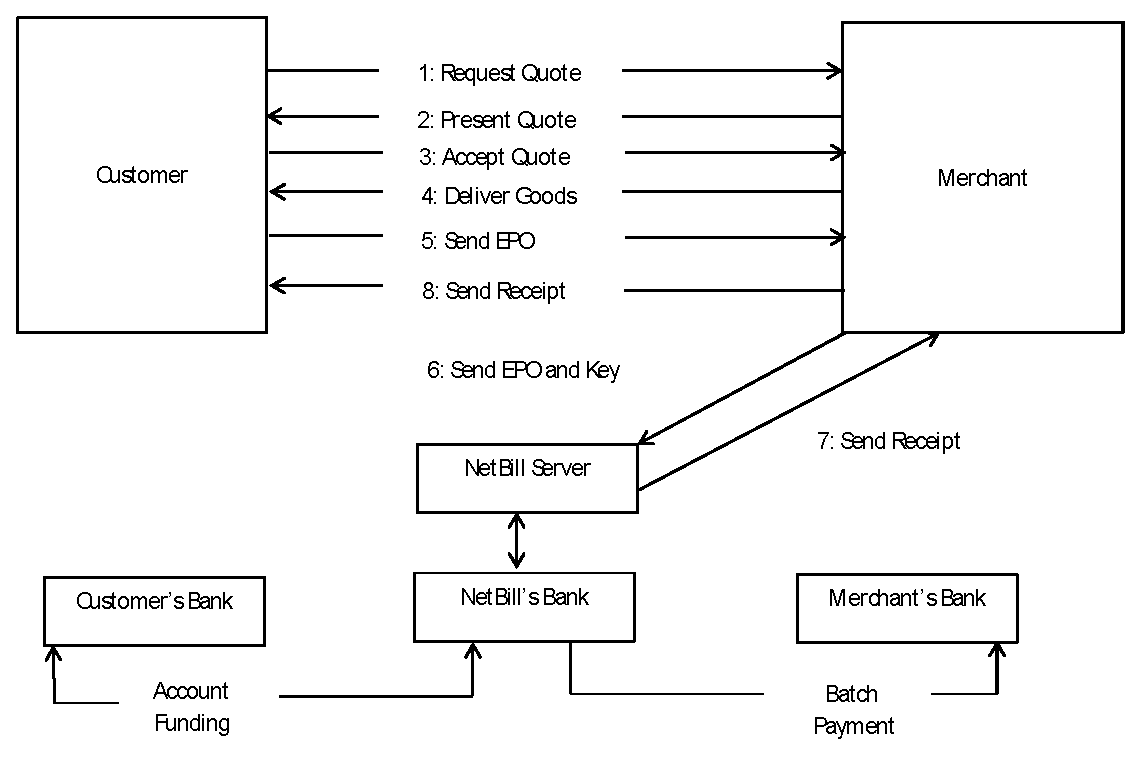
\includegraphics[width=12cm, height=8cm]{figures/figure1.eps}
        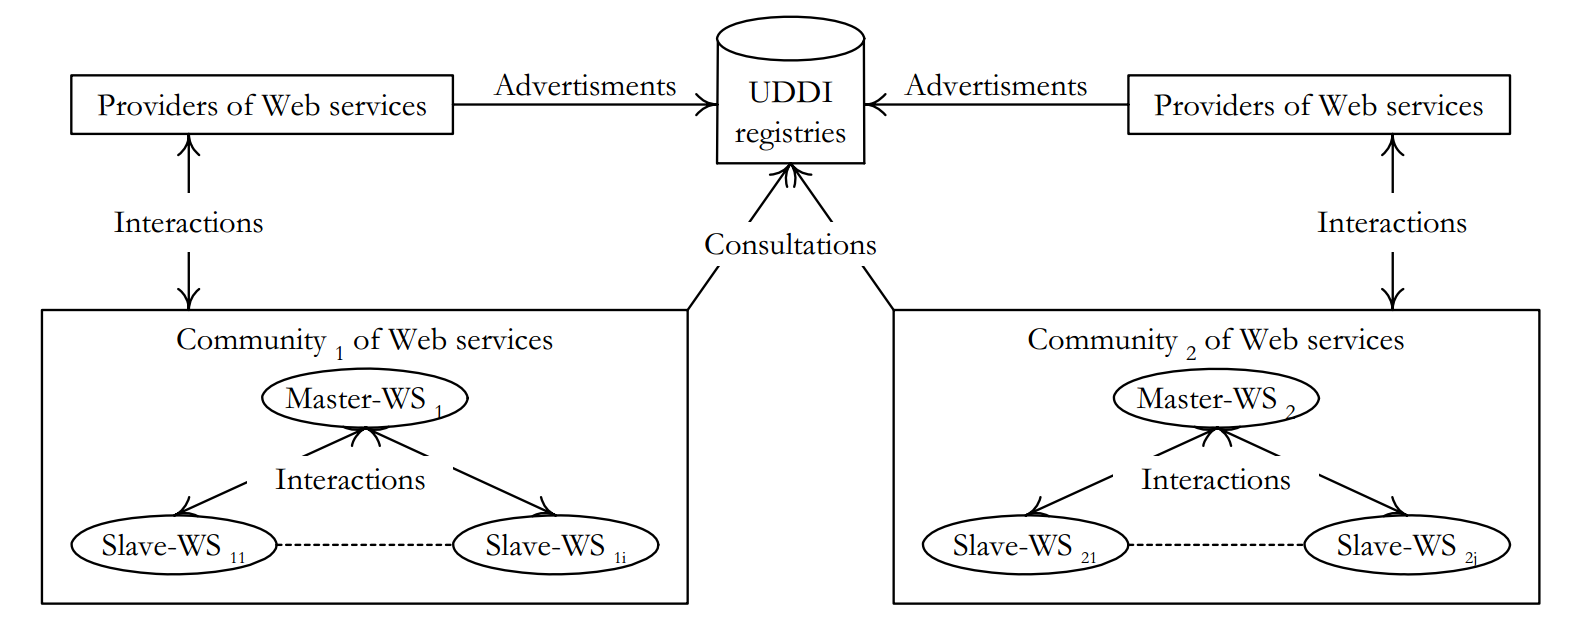
\includegraphics[width=1.0 \columnwidth]{figures/wscommunity2.png}
        %%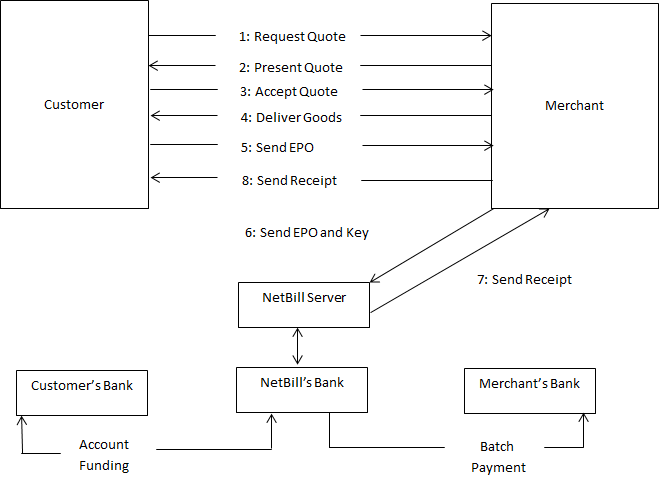
\includegraphics[scale=0.5]{figure1}
        %\caption{The NetBill payment protocol} \label{figure7}
    \end{figure}

    \tiny
    \begin{itemize}
      \item {\color{blue}\lbrack Z. Maamar\rbrack} An Approach to Engineer Communities of Web Services
      \item {\color{blue}\lbrack B. Khosravifar\rbrack} A Game Theoretic Approach for Analyzing the Efficiency of Web Services in Collaborative Networks
      \item {\color{blue}\lbrack E. Lim\rbrack} Using 3-Way Satisfaction for Web Service Selection
      \item {\color{blue}\lbrack A. Liu\rbrack} Coalition Game for Community-based Autonomous Web Services Cooperation
    \end{itemize}                      	      	
\end{frame}

%%%%%%%%%%%%%%%%%%%%%%%%%%%%%%%%%%%%%%%%%%%%%%%%%%%%%%%%%%%%%%%%%%%%%%%%%%%%%%
\subsection{Cooperative Game Theory}

\begin{frame}{Cooperative Game Theory}
  \begin{itemize}
     \item Cooperative games are a branch of game theory that models cooperation or collaboration between agents.
     \begin{itemize}
        \item Cooperation to perform a set of tasks that requires different expertise.
        \item Agents do not have enough resource on their own to perform the tasks.
        \item Examples:
        \begin{itemize}
            \item Robots have the ability to move objects in a plant, but multiple robots are required to move a heavy box.
            \item Transportation domain: agents are trucks, trains, airplanes, ships... a task is a good to be transported.
        \end{itemize}
    \end{itemize}
    \item \textbf{Issues:}
        \begin{itemize}
            \item Coalition formation.
            \item Rewarding members when a task is completed.
        \end{itemize}
  \end{itemize}
\end{frame}

%%%%%%%%%%%%%%%%%%%%%%%%%%%%%%%% frame14 Background and Literature Review %%%%%%%%%%%%%%%%%%%%%%%%%%%%%%%%%%%%%
%%%%%%%%%%%%%%%%%%%%%%%%%%%%%%%%%%%%%%%%%%%%%%%%%%%%%%%%%%%%%%%%%%%%%%%%%%%%%%
\begin{frame}{Cooperative Game Theory}
    %\begin{itemize}
%         \item Cooperative games are a branch of game theory that models cooperation or collaboration between agents within coalitions.
%    \end{itemize}
    \begin{definition} [Coalition]~\\
       We have a population $N$ of $n$ agents, A coalition $C$ is a set of agents: $C \in 2^N$.
        \begin{itemize}
            \item $N$ is the set of all agents (or players)
            \item $v:2^N \rightarrow R$ is the \emph{valuation function}. For $C \subseteq N$, $v(C)$ is the value obtained by the coalition $C$
        \end{itemize}
    \end{definition}

    \begin{itemize}
        \item \textbf{Problem:} Given a game $(N,v)$, and assuming all agents in $N$ want to cooperate, how to distribute the gain among the agents?
        \item \textbf{Solution:} a payoff distribution $x \in R^n$ that provides a value to individual agents.

%        \begin{itemize}
%            \item What are the interesting properties that $x$ should satisfy?
%            \item How to determine the payoff vector $x$?
%        \end{itemize}

    \end{itemize}
\end{frame}

%%%%%%%%%%%%%%%%%%%%%%%%%%%%%%%%%%%%%%%%%%%%%%%%%%%%%%%%%%%%%%%%%%%%%%%%%%%%%%
%\begin{frame}{Transferable and Non Transferable Utility Games}
%    \begin{itemize}
%        \item \textbf{Games with Transferable Utility (TU games)}
%        \begin{itemize}
%            \item Utility is worth the same for all agents.
%            \item Utility can be {\color{red} compared} or {\color{red} transferred} between agents.
%            \item Irrespective of the division of the coalitional payoff.
%            \begin{itemize}
%                \item In that case members of the coalition enjoy the same total utility.
%            \end{itemize}
%        \end{itemize}
%
%
%        \begin{definition} [Valuation or Characteristic Function]\label{dfn:valuationfunction}
%            A \emph{valuation function v} associates a real number $v(C)$ to any subset $C \subseteq N$, i.e., $v:2^N \rightarrow R$ \\
%            A {\color{blue}\emph{TU game}} is a pair $(N,v)$ where $N$ is a set of agents and where $v$ is a valuation function.
%        \end{definition}
%
%
%
%        \item \textbf{Games with Non Transferable Utility (NTU games)} \\
%            Agents have different preferences over coalitions and rewards. Non-monetary rewards, i.e. item allocation type of problems where items have %different values for different players.
%    \end{itemize}

%\end{frame}
%%%%%%%%%%%%%%%%%%%%%%%%%%%%%%%%%%%%%%%%%%%%%%%%%%%%%%%%%%%%%%%%%%%%%%%%%%%%%%
\begin{frame}{Example: A community of landlords and farmers}
    \begin{figure}[htbp]
        \centering
        %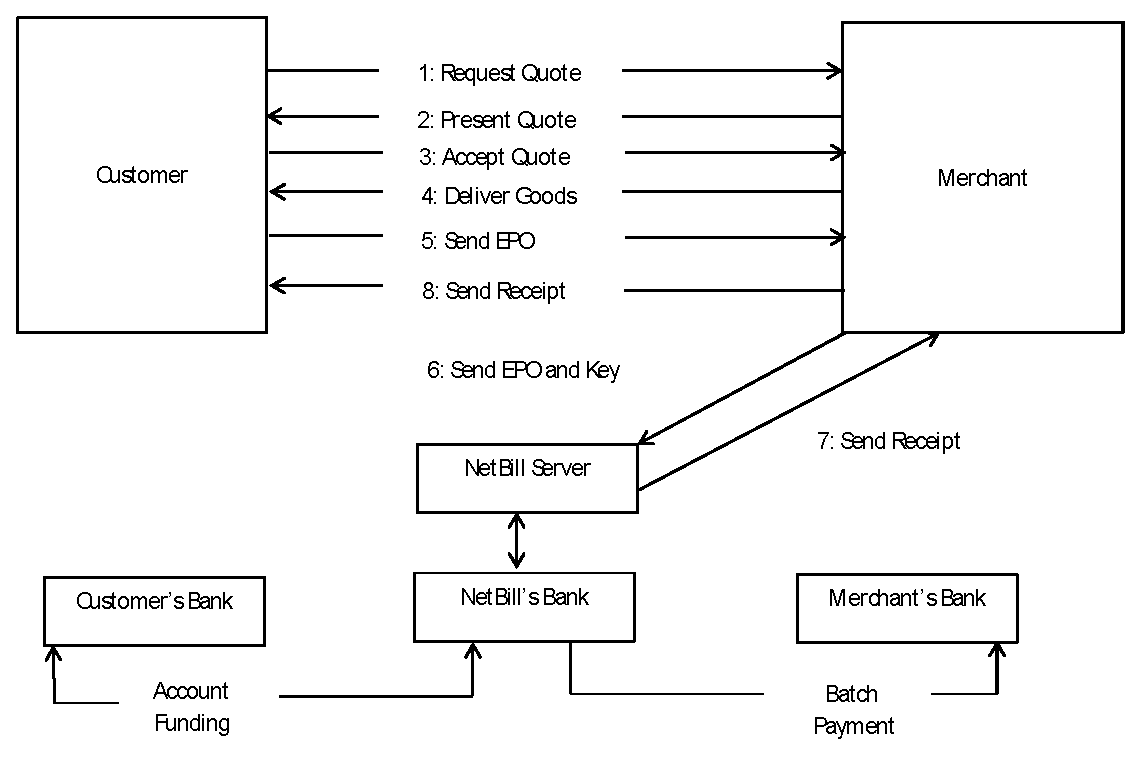
\includegraphics[width=12cm, height=8cm]{figures/figure1.eps}
        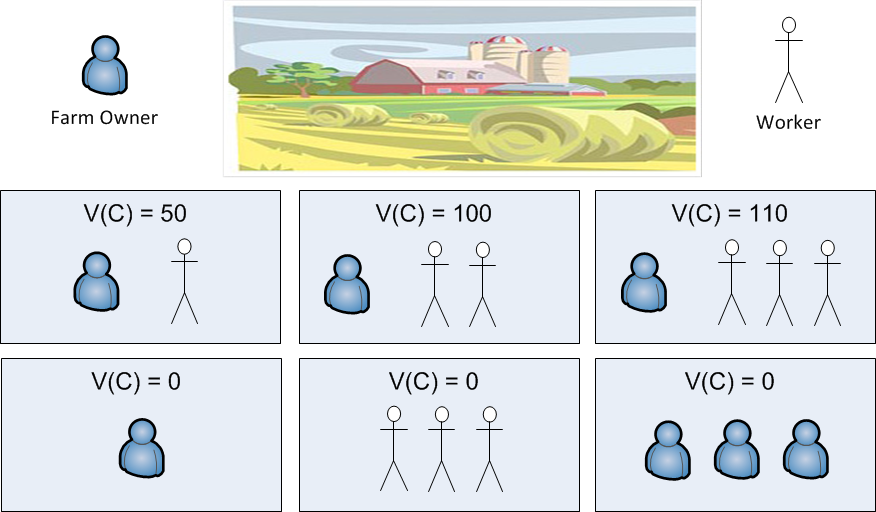
\includegraphics[width=0.9 \columnwidth]{figures/community_farm.png}
        %%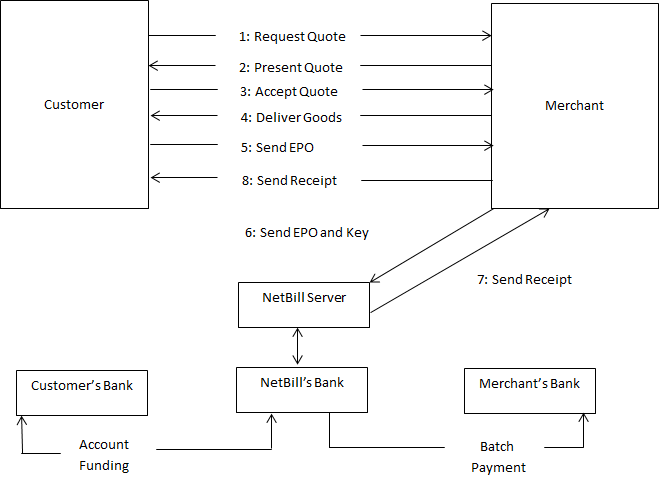
\includegraphics[scale=0.5]{figure1}
        %\caption{The NetBill payment protocol} \label{figure7}
    \end{figure}
\end{frame}
%%%%%%%%%%%%%%%%%%%%%%%%%%%%%%%%%%%%%%%%%%%%%%%%%%%%%%%%%%%%%%%%%%%%%%%%%%%%%%%
\begin{frame}{Some Properties of Valuation Functions}
    $\forall C_1,C_2 \subseteq N | C_1 \bigcap C_2 = \emptyset, i \in N, i \notin C_1$
    \begin{itemize}
        \item {\color{blue} Additive:} $v(C_1 \bigcup C_2) = v(C_1) + v(C_2)$
        \item {\color{blue} Super additive:} $v(C_1 \bigcup C_2) \geq v(C_1) + v(C_2)$ This is satisfied is many applications, or bigger coalitions will not form.
        \item {\color{blue} Weekly super additive:} $v(C_1 \bigcup \{i\}) \geq v(C_1) + v(\{i\})$
        \item {\color{red} Subadditive:} $v(C_1 \bigcup C_2) \leq v(C_1) + v(C_2)$
    \end{itemize}

    $\forall C_1,C_2 \subseteq N$
    \begin{itemize}
        \item {\color{blue} Convex:} $v(C_1 \bigcup C_2) \geq v(C_1) + v(C_2) - v(C_1 \bigcap C_2)$. Convexity has important properties in cooperative game theory solution concepts.
    \end{itemize}
\end{frame}
%%%%%%%%%%%%%%%%%%%%%%%%%%%%%%%%%%%%%%%%%%%%%%%%%%%%%%%%%%%%%%%%%%%%%%%%%%%%%%
\begin{frame}{Solution Properties}
    Let $x \in R^n$ be a solution of the coalition game $(N,v)$
    \begin{itemize}
        \item {\color{blue} Feasible solution:} $\sum_{i \in N} x(i) \leq v(N)$
        \item {\color{blue} Efficiency:} $\sum_{i \in N} x(i) = v(N)$
        \begin{itemize}
            \item the payoff distribution is an allocation of the entire worth of the grand coalition to all agents.
        \end{itemize}
        \item {\color{blue} Individual rationality:} $\forall i \in N, x(i) \geq v(\{i\})$
        \begin{itemize}
            \item player obtains at least its self-value of payoff.
        \end{itemize}
        \item {\color{blue} Group rationality:} $\forall C \subseteq N, \sum_{i \in N} x(i) \geq v(C)$
    \end{itemize}

    \vspace{0.2cm}

    An {\color{blue} imputation} is a payoff distribution $x$ that is efficient and individual rational.

\end{frame}
%%%%%%%%%%%%%%%%%%%%%%%%%%%%%%%%%%%%%%%%%%%%%%%%%%%%%%%%%%%%%%%%%%%%%%%%%%
%\begin{frame}{Stability}
%    \begin{itemize}
%        \item We all want to work together and get $v(N)$, but we all have different views about how to share the fruits of our work. We can use the values of other coalitions as arguments in favor of a distribution.
%        \item A condition for a coalition to form:
%            {\color{blue}all} agents prefer to be in it. i.e., none of the participants wishes she were in a different coalition or by herself {\color{blue} $\Rightarrow Stability$ }
%        \item The {\color{blue} core} is a stability concept for which no agents prefer to deviate to form a different coalition.
%    \end{itemize}
%\end{frame}

%%%%%%%%%%%%%%%%%%%%%%%%%%%%%%%%%%%%%%%%%%%%%%%%%%%%%%%%%%%%%%%%%%%%%%%%%%%%%%%
\begin{frame} {Solution Concepts: Core}
    The core relates to the stability of the grand coalition: \\ No group of agents has any incentive to change coalition.
    \begin{definition}[$Core$ of a Game $(N,v)$]\label{dfn:core}
        Let $(N,v)$ be a cooperative game, and assume they form the coalition $N$. The core of $(N,v)$ is the set:
        \vspace{0.1cm}
        \begin{center}
            $Core(N,v) = \{x \in R^n | x$ is a group rational imputation$\}$
        \end{center}
        Equivalently,
        \vspace{0.1cm}
        \begin{center}
            $Core(N,v) = \{x \in R^n | x(N) \leq v(N) \wedge x(C) \geq v(C), \forall C \subseteq N\}$ \\
        \end{center}
        \small{$x(N) = \sum_{i \in N} x(i)$}
    \end{definition}

    \begin{itemize}
       \item The coalition is stable $\Leftrightarrow$ The core is not empty
    \end{itemize}

\end{frame}
%%%%%%%%%%%%%%%%%%%%%%%%%%%%%%%%%%%%%%%%%%%%%%%%%%%%%%%%%%%%%%%%%%%%%%%%%%%%%%%
%\begin{frame} {Example: Core}
%
%    \begin{center}
%      $N = \{1,2\}$ \\
%      $v(\{1\}) = 5, v(\{2\}) = 5$ \\
%      $v(\{1,2\}) = 20$ \\
%    \end{center}
%
%    $Core(N,n) = \{(x_1,x_2) \in R^2 | x_1 \geq 5, x_2 \geq 5, x_1 + x_2 = 20\}$
%
%    \begin{figure}[htbp]
%        \centering
%        %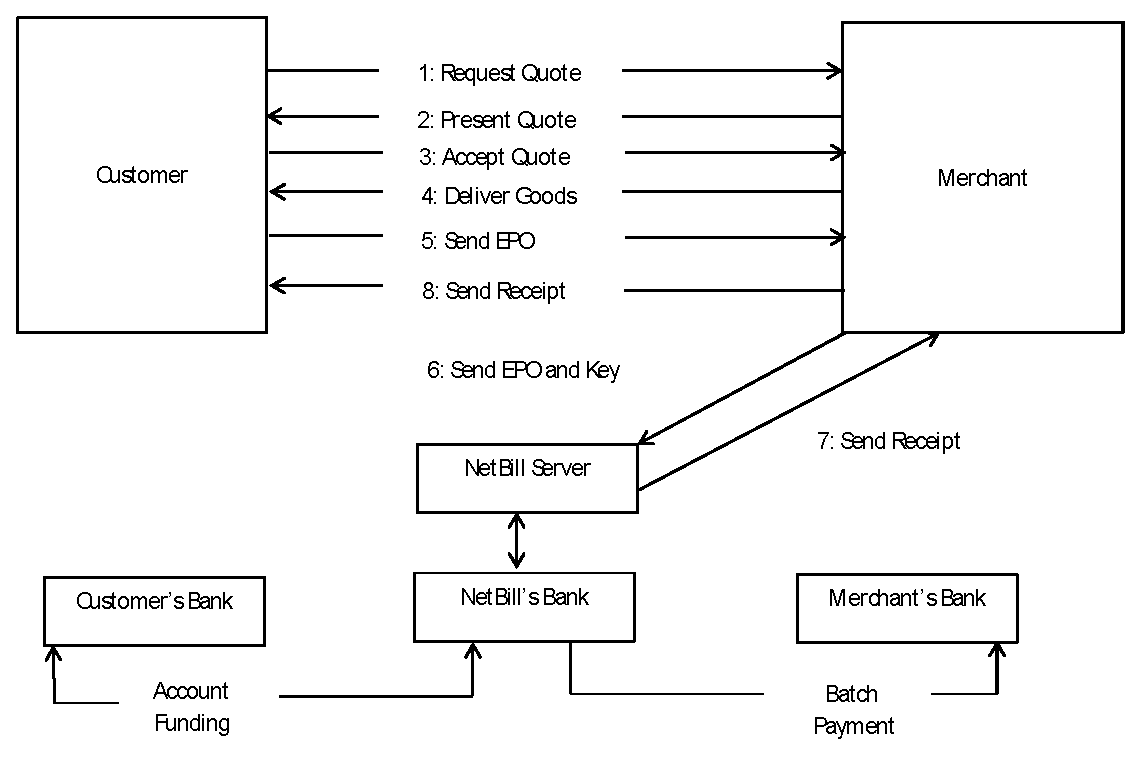
\includegraphics[width=12cm, height=8cm]{figures/figure1.eps}
%        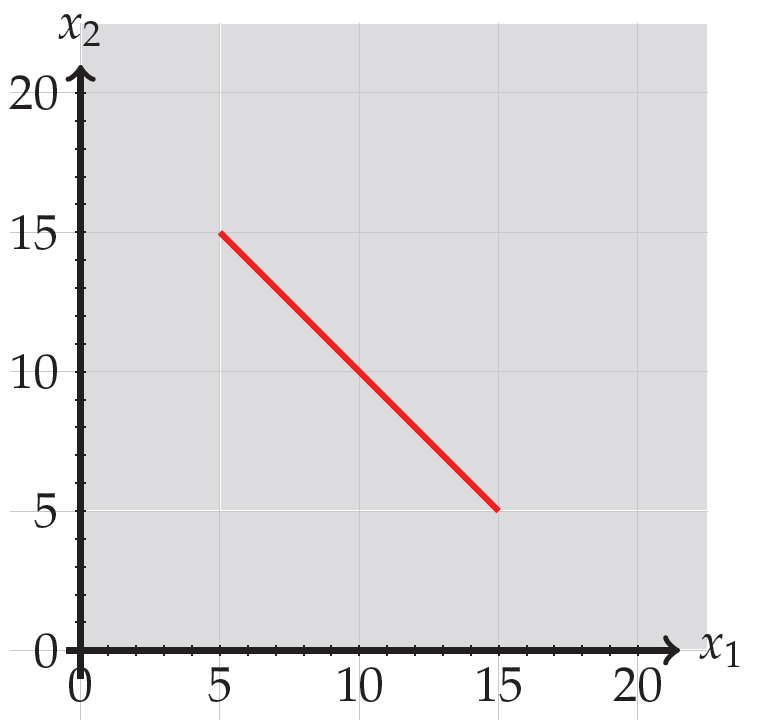
\includegraphics[width=0.3 \columnwidth]{figures/coreex1.png}
%        %%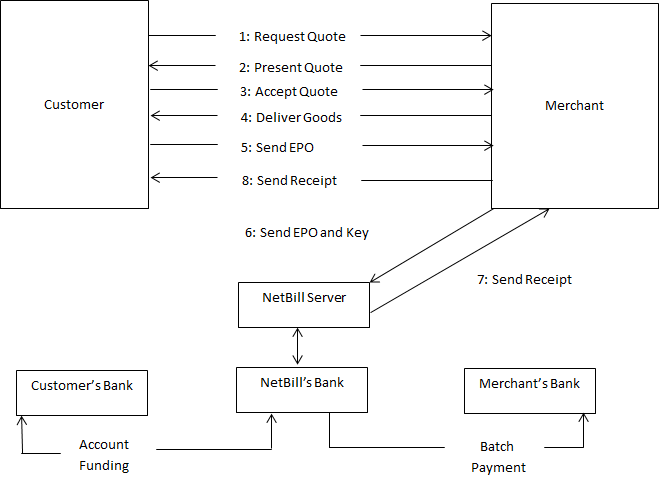
\includegraphics[scale=0.5]{figure1}
%        %\caption{The NetBill payment protocol} \label{figure7}
%    \end{figure}
%
%    The core may not be fair: the core only considers stability.
%
%\end{frame}
%%%%%%%%%%%%%%%%%%%%%%%%%%%%%%%%%%%%%%%%%%%%%%%%%%%%%%%%%%%%%%%%%%%%%%%%%%%%%
\begin{frame}{Solution Concepts: Shapley Value}
    \begin{definition} [Marginal Contribution]\label{dfn:marginalcontribution}
        The {\color{blue}marginal contribution} of agent $i$ for a coalition $C \subseteq N \backslash \{i\}$ is $mc_i(C) = v(C \cup \{i\}) - v(C)$
    \end{definition}

    \begin{itemize}
        \item By considering average marginal contribution over all possible subsets of coalitions, we can achieve a fair distribution.\\
        \item Let $\prod(N)$ denote the set of all permutations of the sequence $(1,...n)$. Therefore: $\phi_i(N,v) = \frac{\sum_{\sigma \in \phi_i(N)}}{mc(\sigma)}$
    \end{itemize}

    \begin{definition} [Shapley Value]\label{dfn:shapleyvalue}
        Given a coalitional game $(N,v)$, the Shapley value of player $i$ is given by: \\
        $\phi_i(N,v) = \sum_{S \subseteq N \backslash \left\{i\right\} } \frac{|S|! (|N|-|S|-1)!}{|N|!} (v(S \cup \left\{i\right\}) - v(S))$
    \end{definition}
\end{frame}
%%%%%%%%%%%%%%%%%%%%%%%%%%%%%%%%%%%%%%%%%%%%%%%%%%%%%%%%%%%%%%%%%%%%%%%%%%%%%%%
\begin{frame}{Some Properties}
    \begin{itemize}
        \item The core set can be empty or have many solutions.
        \item Shapley value always exists and is unique.
        \item When the valuation function is {\color{blue}superadditive}, the Shapley value is {\color{blue}individually rational}, i.e., it is an imputation.
        \item When the valuation function is {\color{blue}convex}, the Shapley value is also group rational, hence, it is in the {\color{blue}core}.
        \item A convex game has a non-empty core.
        \item Core and Shapley value are combinatorial problems.
    \end{itemize}
\end{frame}

%%%%%%%%%%%%%%%%%%%%%%%%%%%%%%%%%%%%%%%%%%%%%%%%%%%%%%%%%%%%%%%%%%%%%%%%%%%%%%%


%%%%%%%%%%%%%%%%%%%%%%%%%%%%%%%%%%%%%%%%%%%%%%%%%%%%%%%%%%%%%%%%%%%%%%%%%%%%%%
%%%%%%%%%%%%%%%%%%%%%%%%%%%%%%%%%%%%%%%%%%%%%%%%%%%%%%%%%%%%%%%%%%%%%%%%%%%%%%%
\section{Proposed Research}
\begin{frame}{Presentation Outline}
    \begin{itemize}
     	\itemsep=.5cm
    	\item Introduction
    	\item Background and Literature Review
    	\item {\bf Proposed Research}
    	\item Conclusion and Feature Work
    \end{itemize}
\end{frame}
%%%%%%%%%%%%%%%%%%%%%%%%%%%%%%%% frame16 Proposed Research %%%%%%%%%%%%%%%%%%%%%%%%%%%%%%%%%%%%%


%%%%%%%%%%%%%%%%%%%%%%%%%%%%%%%%%%%%%%%%%%%%%%%%%%%%%%%%%%%%%%%%%%%%%%%%%%%%%%%
\begin{frame}{Efficient Community Formation for Web Services}
    \begin{figure}[htbp]
        \centering
        %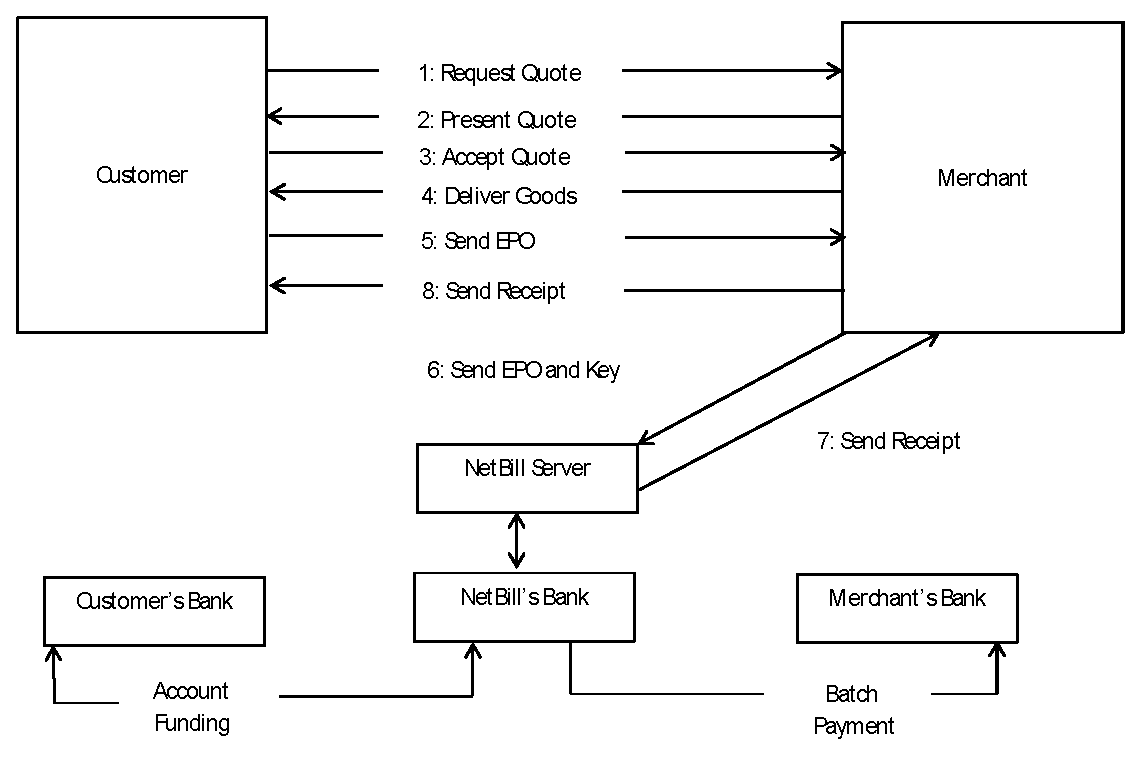
\includegraphics[width=12cm, height=8cm]{figures/figure1.eps}
        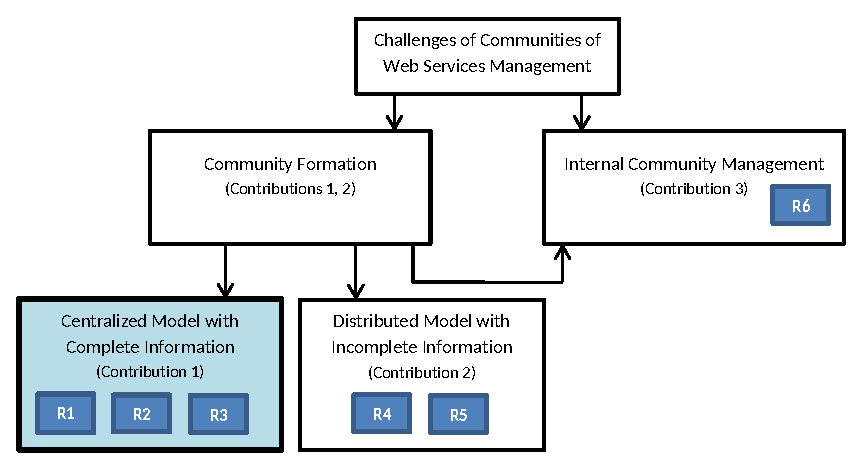
\includegraphics[width=0.9 \columnwidth]{figures/model_c1.eps}
        %%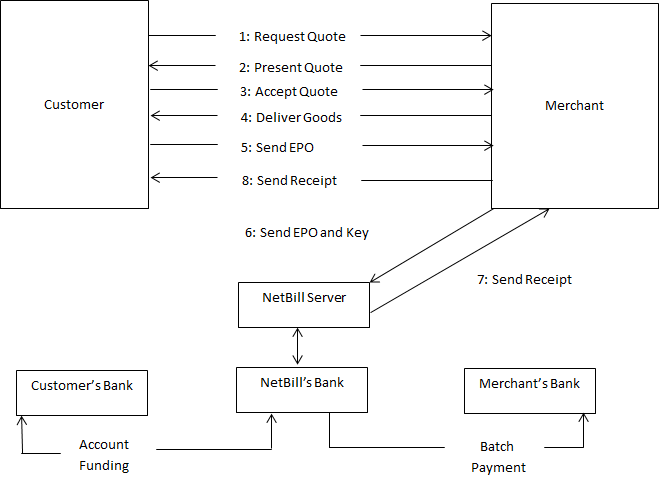
\includegraphics[scale=0.5]{figure1}
        %\caption{The NetBill payment protocol} \label{figure7}
    \end{figure}
\end{frame}
%%%%%%%%%%%%%%%%%%%%%%%%%%%%%%%%%%%%%%%%%%%%%%%%%%%%%%%%%%%%%%%%%%%%%%%%%%%%%%%


%%%%%%%%%%%%%%%%%%%%%%%%%%%%%%%%%%%%%%%%%%%%%%%%%%%%%%%%%%%%%%%%%%%%%%%%%%%%%%%
\subsection{Problem Formulation and Modeling}

\begin{frame}{Problem Formulation and Modeling}
    \begin{itemize}
        \item Communities of web services are robust service providers with well established market share and reputation.
        \item The community is characterized by a request rate $R_C$.
        \item Web services can perform tasks with some throughput rate ($Th_{ws}$).
        \item Web services come with different values of $QoS_{ws}$ for different metrics.
    \end{itemize}
\end{frame}

%%%%%%%%%%%%%%%%%%%%%%%%%%%%%%%%%%%%%%%%%%%%%%%%%%%%%%%%%%%%%%%%%%%%%%%%%%%%%%%
\begin{frame}{Task Distribution}
    \begin{itemize}
        \item Our model uses a slightly modified \emph{weighted fair queuing} method for task distribution rather than Contract-Net.
        \item All the input flow is multiplexed among different web services with weights proportional to their throughput value ($Th_{ws}$).
        \item Queues will happen if $R_C$ is more than the summation of web services throughput.
        \item Weighted task rate: $R_C \times \frac{Th_{ws}}{\sum_{ws}{Th_{ws}}}$ or $Th_{ws}$
    \end{itemize}
    \begin{figure}[htbp]
        \centering
        %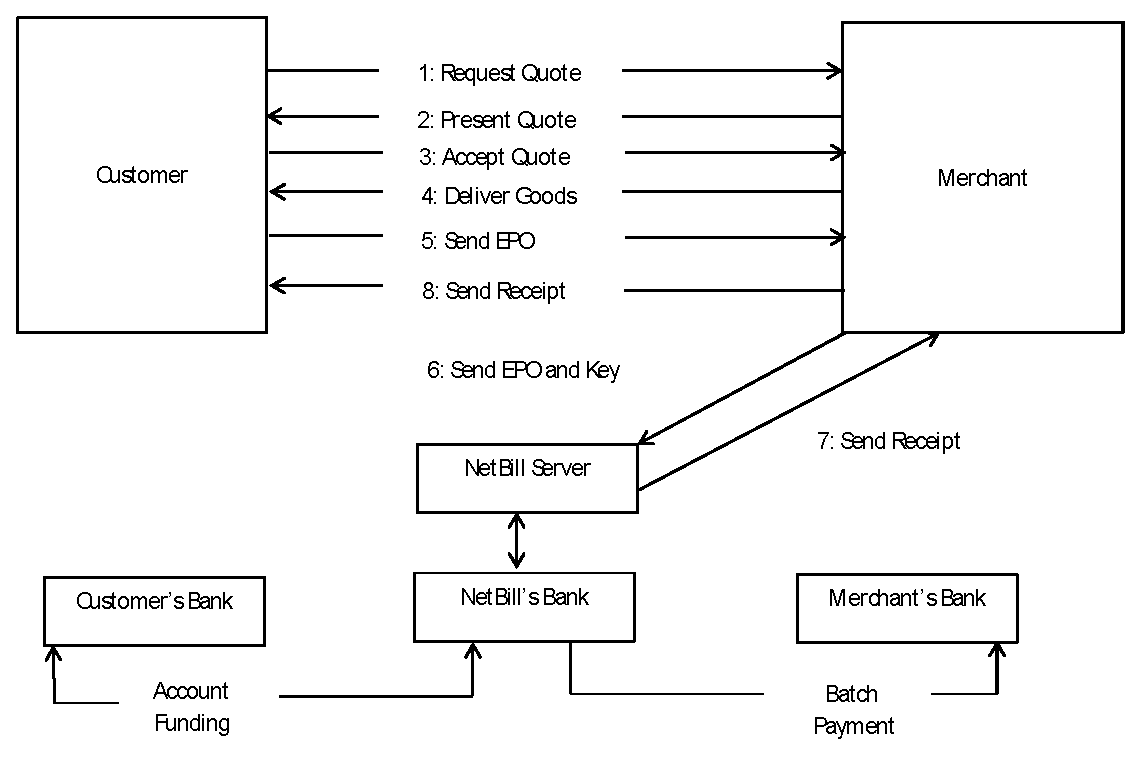
\includegraphics[width=12cm, height=8cm]{figures/figure1.eps}
        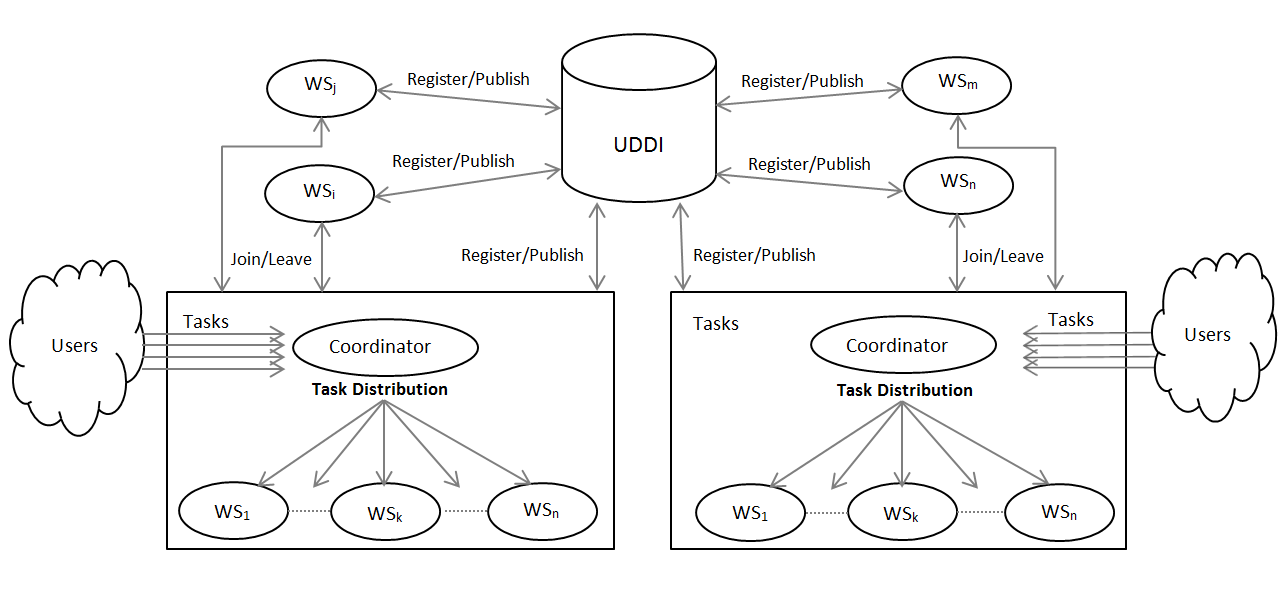
\includegraphics[width=0.8 \columnwidth]{figures/community.png}
        %%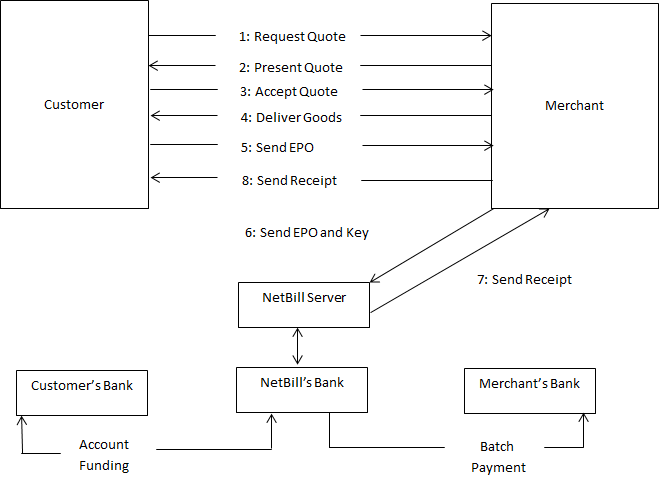
\includegraphics[scale=0.5]{figure1}
        %\caption{The NetBill payment protocol} \label{figure7}
    \end{figure}
\end{frame}

%%%%%%%%%%%%%%%%%%%%%%%%%%%%%%%%%%%%%%%%%%%%%%%%%%%%%%%%%%%%%%%%%%%%%%%%%%%%%%%
\begin{frame}{Community Revenue}
    \begin{itemize}
        \item Maximum potential output of a community:
            \begin{equation*}
                PO(C) = \sum_{ws \in C}{(T_{ws} \times QoS_{ws})}
            \end{equation*}
        \item if $\sum_{ws}{Th_{ws}} > R_C$, the community cannot perform at its maximum potential.
        \item Actual output:
            \begin{equation}\label{out_c}
                Out(C) = \left\{
                  \begin{array}{l l}
                    PO(C) & \quad \text{if $\sum_{ws}{Th_{ws}} \leq R_{C}$}\\
                    PO(C) \times \frac{R_{C}}{\sum_{ws}{Th_{ws}}} & \quad \text{if $\sum_{ws}{Th_{ws}} > R_{C}$}
                  \end{array} \right.
            \end{equation}
    \end{itemize}
\end{frame}

%%%%%%%%%%%%%%%%%%%%%%%%%%%%%%%%%%%%%%%%%%%%%%%%%%%%%%%%%%%%%%%%%%%%%%%%%%%%%%%
\begin{frame}{Example 1}
    \begin{table}[!t]
    \renewcommand{\arraystretch}{1.3}
    % if using array.sty, it might be a good idea to tweak the value of
    % \extrarowheight as needed to properly center the text within the cells
    \label{example_1}
    \centering
    \begin{tabular}{c c c c}
    \hline
    $WS$ & $QoS_{ws}$ & $Th_{ws}$ & $Th_{ws} \times QoS_{ws}$\\
    \hline
    1 & 0.8 & 4 & 3.2\\
    2 & 0.8 & 5 & 4.0\\
    3 & 0.8 & 3 & 2.4\\
    \hline
    \end{tabular}
    \end{table}

    \begin{table}[!t]
    \renewcommand{\arraystretch}{1.3}
    % if using array.sty, it might be a good idea to tweak the value of
    % \extrarowheight as needed to properly center the text within the cells
    % \caption{Three web services}
    \label{example_1_2}
    \centering
    \begin{tabular}{c c || c c}
    \hline
    Community & Worth & Community & Worth\\
    \hline
    $\left\{1\right\}$ & 3.2 & $\left\{1,2\right\}$ & 7.2\\
    $\left\{2\right\}$ & 4.0 & $\left\{1,3\right\}$ & 5.6\\
    $\left\{3\right\}$ & 2.4 & $\left\{2,3\right\}$ & 6.4\\
    $\left\{1,2,3\right\}$ & 8.0\\
    \hline
    Community $R_C$: 10\\
    \hline
    \end{tabular}
    \end{table}
\end{frame}

%%%%%%%%%%%%%%%%%%%%%%%%%%%%%%%%%%%%%%%%%%%%%%%%%%%%%%%%%%%%%%%%%%%%%%%%%%%%%%%%
%\begin{frame}{Example 2}
%    \begin{table}[!t]
%    \renewcommand{\arraystretch}{1.3}
%    % if using array.sty, it might be a good idea to tweak the value of
%    % \extrarowheight as needed to properly center the text within the cells
%    \label{example_2}
%    \centering
%    \begin{tabular}{c c c c}
%    \hline
%    $WS$ & $QoS_{ws}$ & $Th_{ws}$ & $Th_{ws} \times QoS_{ws}$\\
%    \hline
%    1 & 0.8 & 5 & 4.0\\
%    2 & 0.7 & 6 & 4.2\\
%    3 & 0.7 & 4 & 2.8\\
%    \hline
%    \end{tabular}
%    \end{table}
%
%    \begin{table}[!t]
%    \renewcommand{\arraystretch}{1.3}
%    % if using array.sty, it might be a good idea to tweak the value of
%    % \extrarowheight as needed to properly center the text within the cells
%    % \caption{Three web services}
%    \label{example_2_2}
%    \centering
%    \begin{tabular}{c c || c c}
%    \hline
%    Community & Worth & Community & Worth\\
%    \hline
%    $\left\{1\right\}$ & 4.0 & $\left\{1,2\right\}$ & 7.4\\
%    $\left\{2\right\}$ & 4.2 & $\left\{1,3\right\}$ & 6.8\\
%    $\left\{3\right\}$ & 2.8 & $\left\{2,3\right\}$ & 7.0\\
%    $\left\{1,2,3\right\}$ & 7.3\\
%    \hline
%    Community $R_C$: 10\\
%    \hline
%    \end{tabular}
%    \end{table}
%\end{frame}

%%%%%%%%%%%%%%%%%%%%%%%%%%%%%%%%%%%%%%%%%%%%%%%%%%%%%%%%%%%%%%%%%%%%%%%%%%%%%%%
\begin{frame}{Example 2}
    \begin{table}[!t]
    \renewcommand{\arraystretch}{0.8}
    % if using array.sty, it might be a good idea to tweak the value of
    % \extrarowheight as needed to properly center the text within the cells
    \label{example_3}
    \centering
    \begin{tabular}{c c c c}
    \hline
    $WS$ & $QoS_{ws}$ & $Th_{ws}$ & $\text{\emph{Input Task Rate}}$\\
    \hline
    1 & 0.8 & 10 & 5\\
    2 & 0.8 & 20 & 5\\
    3 & 0.8 & 30 & 5\\
    \hline
    \end{tabular}
    \end{table}

    \begin{table}[!t]
    \renewcommand{\arraystretch}{0.8}
    % if using array.sty, it might be a good idea to tweak the value of
    % \extrarowheight as needed to properly center the text within the cells
    % \caption{Three web services}
    \label{example_3_2}
    \centering
    \begin{tabular}{c c || c c}
    \hline
    Community & Worth & Community & Worth\\
    \hline
    $\left\{C_{ms_1}\right\}$ & 0 & $\left\{C_{ms_2}\right\}$ & 0\\
    $\left\{C_{ms_1}, ws_1\right\}$ & 8 & $\left\{C_{ms_2}, ws_1\right\}$ & 8\\
    $\left\{C_{ms_1}, ws_2\right\}$ & 16 & $\left\{C_{ms_2}, ws_2\right\}$ & 16\\
    $\left\{C_{ms_1}, ws_3\right\}$ & 16 & $\left\{C_{ms_2}, ws_3\right\}$ & 24\\
    $\left\{C_{ms_1}, ws_1, ws_2\right\}$ & 16 & $\left\{C_{ms_2}, ws_1, ws_2\right\}$ & 24\\
    $\left\{C_{ms_1}, ws_1, ws_3\right\}$ & 16 & $\left\{C_{ms_2}, ws_1, ws_3\right\}$ & 32\\
    $\left\{C_{ms_1}, ws_2, ws_3\right\}$ & 16 & $\left\{C_{ms_2}, ws_2, ws_3\right\}$ & 32\\
    $\left\{C_{ms_1}, ws_1, ws_2, ws_3\right\}$ & 16 & $\left\{C_{ms_2}, ws_1, ws_2, ws_3\right\}$ & 32\\
    $\left\{C_{ms_1}, C_{ms_2}, ...\right\}$ & 0 & $\left\{ws_1\right\}$ & 6.8\\
    $\left\{ws_2\right\}$ & 4.2 & $\left\{ws_3\right\}$ & 6.8\\
    \hline
    Community $R_{C_1}$: 20 \\ Community $R_{C_2}$: 40\\
    \hline
    \end{tabular}
    \end{table}
\end{frame}

%%%%%%%%%%%%%%%%%%%%%%%%%%%%%%%% frame19 Proposed Research
%%%%%%%%%%%%%%%%%%%%%%%%%%%%%%%%%%%%%%%%%%%%%%%%%%%%%%%%%%%%%%%%%%%%%%%%%%%%%%%
\subsection{Web Service Cooperative Games}

%%%%%%%%%%%%%%%%%%%%%%%%%%%%%%%%%%%%%%%%%%%%%%%%%%%%%%%%%%%%%%%%%%%%%%%%%%%%%%%
\begin{frame}{Community and Web Service Interaction Model}
    \begin{figure}[htbp]
        \centering
        %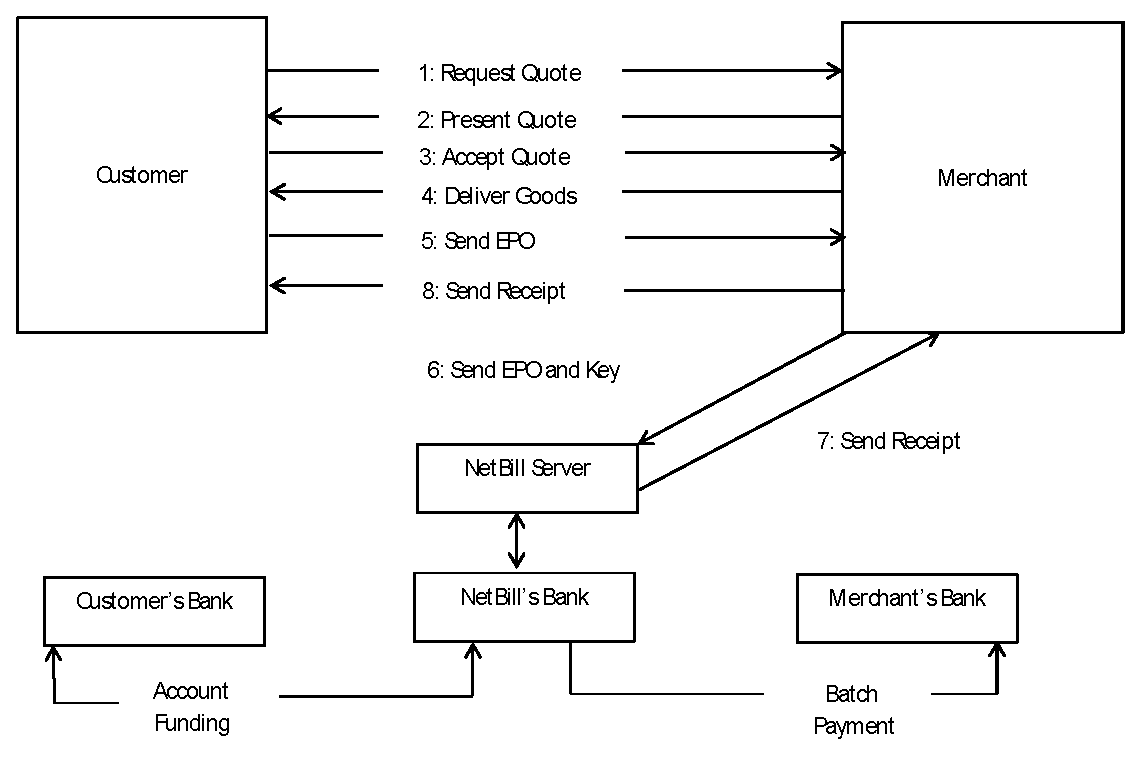
\includegraphics[width=12cm, height=8cm]{figures/figure1.eps}
        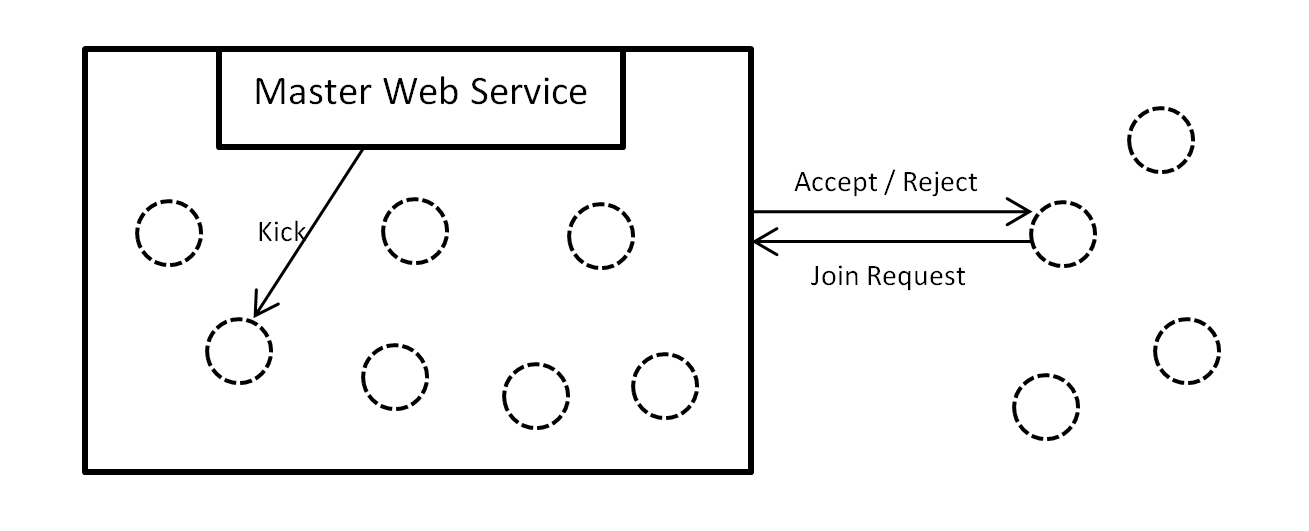
\includegraphics[width=0.8 \columnwidth]{figures/scenario1.png}
        %%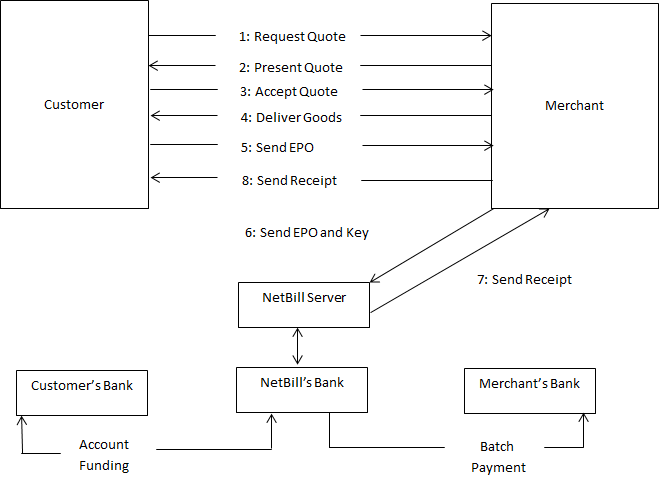
\includegraphics[scale=0.5]{figure1}
        %\caption{The NetBill payment protocol} \label{figure7}
    \end{figure}

    \begin{itemize}
        \item A typical WS community, where web services can join or leave.
        \item $v(C) = Out(C)$.
        \item Membership decision in made based on throughput and QoS of the web services.
        \item Community master needs to get quality web services to keep the community stable, so other web services have no incentive to leave.
    \end{itemize}
       	
\end{frame}
%%%%%%%%%%%%%%%%%%%%%%%%%%%%%%%%%%%%%%%%%%%%%%%%%%%%%%%%%%%%%%%%%%%%%%%%%%%%%%%
\begin{frame}{Community and Web Service Interaction Model}
    \begin{itemize}
        \item Upon receiving membership request, the master web service checks if the coalition will be stable having the new member.
        \item If the game is convex, core exists.
        \item If the game is convex, Shapley value is in core.
        \item Convexity Condition:
        \begin{center}
          $v(A \cup B) \geq v(A) + v(B) - v(A \cap B)$ \\
          $\Leftrightarrow$  \\
          $\forall S,T | S \subseteq T \subseteq N \backslash \left\{i\right\}, \forall i \in N,$ \\
          {\color{blue} $v(S \cup \left\{i\right\}) - v(S) \leq v (T \cup \left\{i\right\}) - v(T)$ }
        \end{center}
        %\item Depth-1 Convexity Check: $O(n)$
        %\item Depth-2 Convexity Check: $O(n^2)$
    \end{itemize}       	
\end{frame}

\begin{frame}{Depth-k Convexity Check}

    \begin{figure}
        \includegraphics<1>[width=0.75 \columnwidth]{figures/depthk1_6.png}
        \includegraphics<2>[width=0.75 \columnwidth]{figures/depthk1_5.png}
        \includegraphics<3>[width=0.75 \columnwidth]{figures/depthk1_4.png}
        \includegraphics<4>[width=0.75 \columnwidth]{figures/depthk1_3.png}
        \includegraphics<5>[width=0.75 \columnwidth]{figures/depthk1_2.png}
        \includegraphics<6>[width=0.75 \columnwidth]{figures/depthk1_1.png}
        \includegraphics<7>[width=0.75 \columnwidth]{figures/depthk2_56.png}
        \includegraphics<8>[width=0.75 \columnwidth]{figures/depthk2_46.png}
        \includegraphics<9>[width=0.75 \columnwidth]{figures/depthk2_45.png}
        \includegraphics<10>[width=0.75 \columnwidth]{figures/depthk2_12.png}
    \end{figure}

    \begin{center}
        $v({\color{blue} S} \cup {\color{green}\left\{i\right\}}) - v({\color{blue} S}) \leq v (T \cup {\color{green}\left\{i\right\}}) - v(T)$ \\
        \only<1>{
            ${\color{black} T = \left\{1,2,3,4,5,6\right\}}$ \\
            ${\color{blue} S = \left\{1,2,3,4,5\right\}}$
        }
        \only<2>{
            ${\color{black} T = \left\{1,2,3,4,5,6\right\}}$ \\
            ${\color{blue} S = \left\{1,2,3,4,6\right\}}$
        }
        \only<3>{
            ${\color{black} T = \left\{1,2,3,4,5,6\right\}}$ \\
            ${\color{blue} S = \left\{1,2,3,5,6\right\}}$
        }
        \only<4>{
            ${\color{black} T = \left\{1,2,3,4,5,6\right\}}$ \\
            ${\color{blue} S = \left\{1,2,4,5,6\right\}}$
        }
        \only<5>{
            ${\color{black} T = \left\{1,2,3,4,5,6\right\}}$ \\
            ${\color{blue} S = \left\{1,3,4,5,6\right\}}$
        }
        \only<6>{
            ${\color{black} T = \left\{1,2,3,4,5,6\right\}}$ \\
            ${\color{blue} S = \left\{2,3,4,5,6\right\}}$
        }
        \only<7>{
            ${\color{black} T = \left\{1,2,3,4,5,6\right\}}$ \\
            ${\color{blue} S = \left\{1,2,3,4\right\}}$
        }
        \only<8>{
            ${\color{black} T = \left\{1,2,3,4,5,6\right\}}$ \\
            ${\color{blue} S = \left\{1,2,3,5\right\}}$
        }
        \only<9>{
            ${\color{black} T = \left\{1,2,3,4,5,6\right\}}$ \\
            ${\color{blue} S = \left\{1,2,3,6\right\}}$
        }
        \only<10>{
            ${\color{black} T = \left\{1,2,3,4,5,6\right\}}$ \\
            ${\color{blue} S = \left\{3,4,5,6\right\}}$
        }

    \end{center}

    \begin{itemize}
        \only<1,2,3,4,5,6>{
            \item Depth-1 Convexity Check: $O(n)$
        }
        \only<7,8,9,10>{
            \item Depth-1 Convexity Check: $O(n)$
            \item Depth-2 Convexity Check: $O(n^2)$
        }

        %\item \only<1>{First Image}\only<2>{Second Image}
    \end{itemize}

\end{frame}

%
%\begin{frame}{Scenario Two: Web Services and Many Communities}
%    \begin{itemize}
%        \item Based on Coalition Structure theory
%        \begin{itemize}
%            \item Which coalitions to form?
%            \item Stability in coalition structure is a partition of players, where no other partition can provide all agents with better utility.
%            \item Social welfare: $\operatorname*{arg\,max}_{CS} v(CS)$ where $v(CS) = \sum_{C \in CS}v(C)$.
%        \end{itemize}
%        \item Has to be distributed not centralized.
%        \item Merge and Split Algorithm {\footnotesize{\color{blue}{(Krzysztof R. Apt and Andreas Witzel)}}}
%        \begin{itemize}
%            \item Is iterative
%            \item Converges to a final partition
%        \end{itemize}
%    \end{itemize}
%    \begin{figure}[htbp]
%        \centering
%        %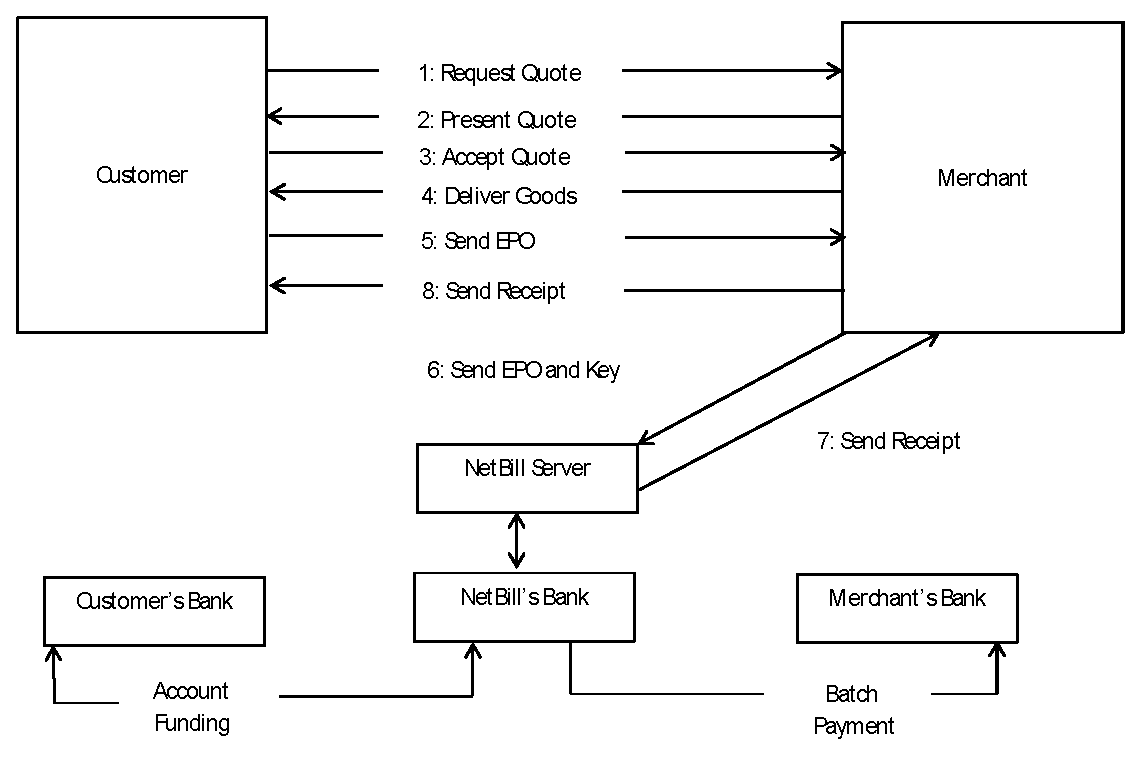
\includegraphics[width=12cm, height=8cm]{figures/figure1.eps}
%        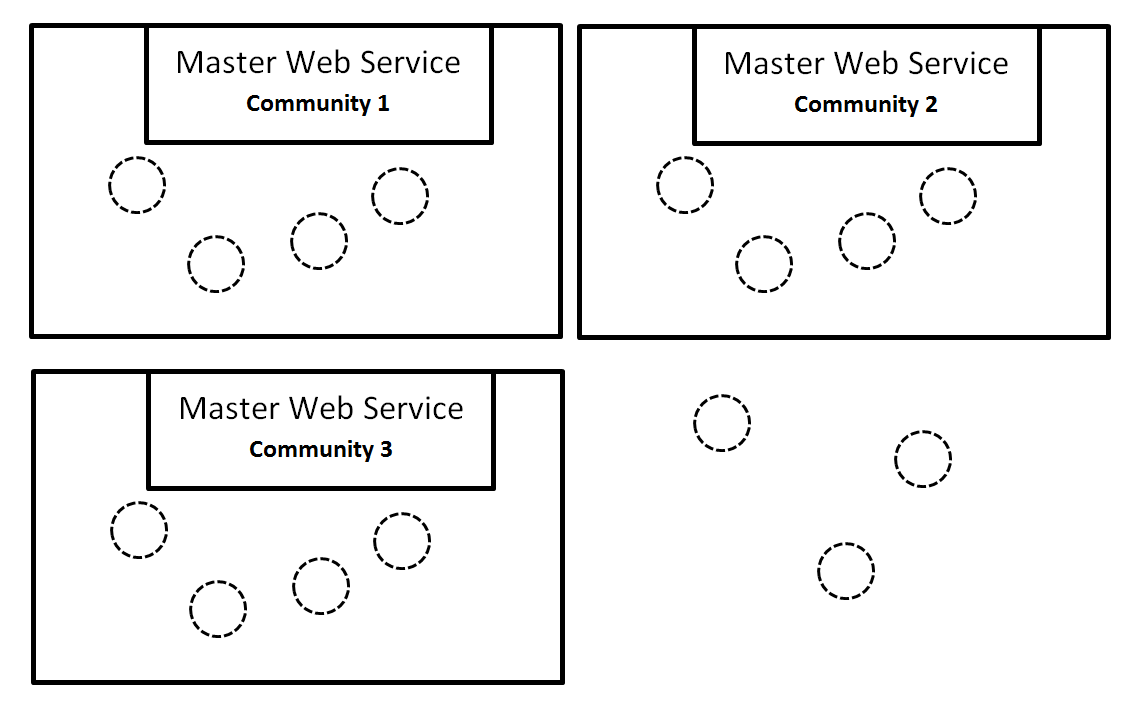
\includegraphics[width=0.5 \columnwidth]{figures/scenario2.png}
%        %%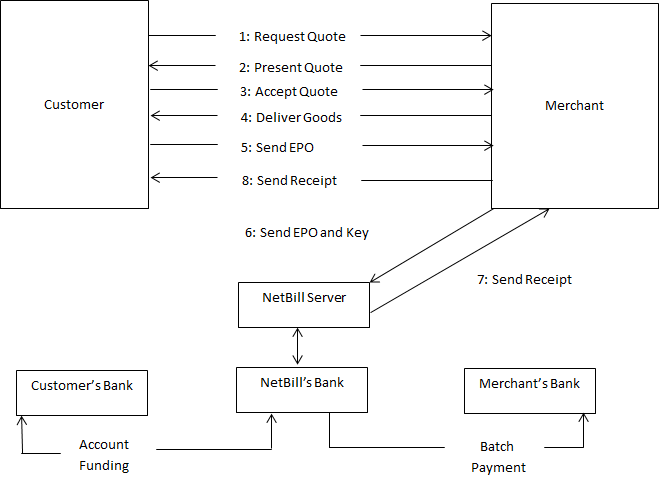
\includegraphics[scale=0.5]{figure1}
%        %\caption{The NetBill payment protocol} \label{figure7}
%    \end{figure}       	
%\end{frame}


%%%%%%%%%%%%%%%%%%%%%%%%%%%%%%%%%%%%%%%%%%%%%%%%%%%%%%%%%%%%%%%%%%%%%%%%%%%%%%
%\subsection{Experimental Results}
\begin{frame}{Experimental Results}

    \begin{figure}[!t]
    \centering
    %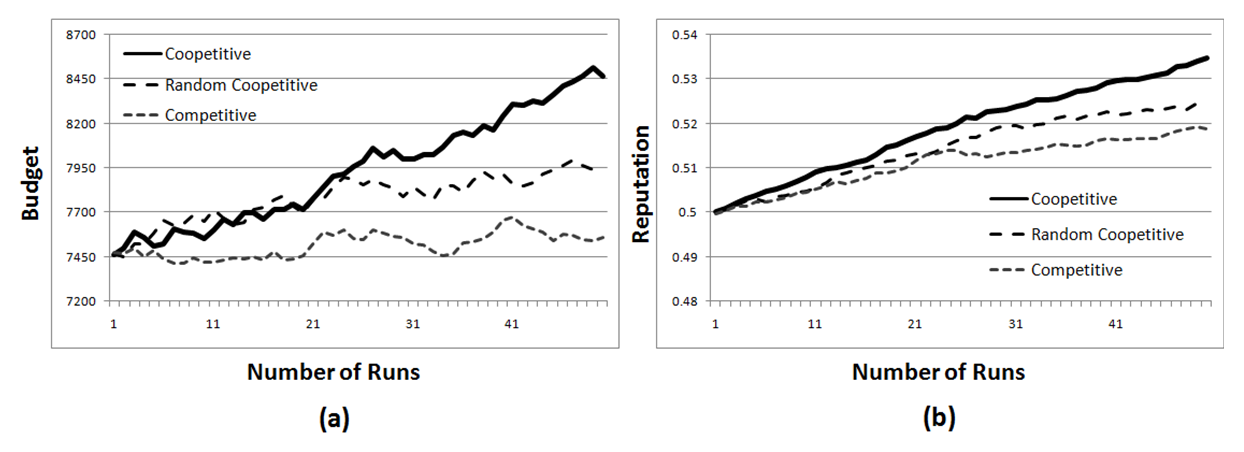
\includegraphics[scale=0.6]{graph1Final+.eps}
    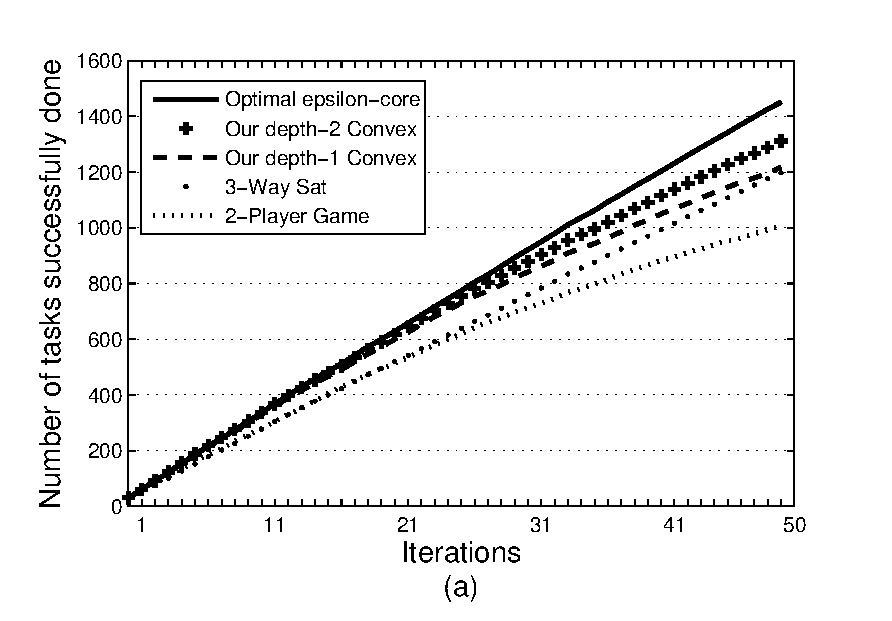
\includegraphics[width=2.1in]{figures/task_done_opt.eps}
    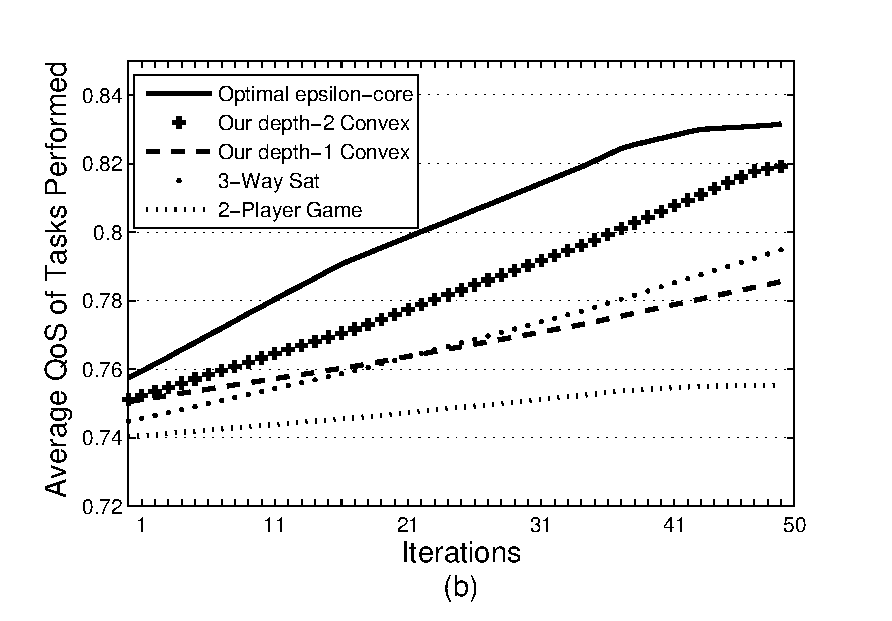
\includegraphics[width=2.1in]{figures/task_qos_opt.eps}
    \caption{Part (a): Cumulative number of requests successfully
    answered. Part (b): Average QoS of requests performed.}
    \label{performanceall}
    \end{figure}

\end{frame}
%%%%%%%%%%%%%%%%%%%%%%%%%%%%%%%%%%%%%%%%%%%%%%%%%%%%%%%%%%%%%%%%%%%%%%%%%%%%%%

%%%%%%%%%%%%%%%%%%%%%%%%%%%%%%%%%%%%%%%%%%%%%%%%%%%%%%%%%%%%%%%%%%%%%%%%%%%%%%%
\subsection{Taxation, Subsiding and Stability}
\begin{frame}{Improving Community Stability}
    \begin{itemize}
        \item The core may not always be non-empty, core is a strong condition.
        \item The optimal solution concepts will attract only enough services satisfying input task rate, not more.
        \item In case of web service failure, a portion of tasks will not be handled efficiently until replacement is found.
        \item By imposing cost on deviation or subsiding the community, its possible to attract more web services and keep the community stable.
        \item Will be cost efficient in case of web service failure, or for replacing web services dropping in QoS metrics as they advertised.
        \item \emph{Taxation} would need agreement between all communities (needs a centralized approach), however \emph{subsiding} can be done within communities in distributed manner.
    \end{itemize}
\end{frame}
%%%%%%%%%%%%%%%%%%%%%%%%%%%%%%%%%%%%%%%%%%%%%%%%%%%%%%%%%%%%%%%%%%%%%%%%%%%%%%%

%%%%%%%%%%%%%%%%%%%%%%%%%%%%%%%%%%%%%%%%%%%%%%%%%%%%%%%%%%%%%%%%%%%%%%%%%%%%%%%
\begin{frame}{Taxation and Subsiding}
    \begin{itemize}
        \item Least Core
        \begin{itemize}
            \item $\forall S \subseteq N, \sum_{x_i \in S} x_i \geq v(S) - \epsilon$
            \item $\epsilon$-core relaxes the core condition.
        \end{itemize}
        \item Taxation in Reliability Games \small $[Y. Bachrach, E. Elkind, 2009]$

        \item Taxation and Cost of Stability \small $[R. Meir, J. S. Rosenchein, 2011]$

        \item Taxation in Anonymous Games \small $[Y. Zick, M. Polukarov, 2013]$

        \item Relative Core
        \begin{itemize}
            \item $\lambda v(C)$ is divided among players.
            \item relative $\lambda$-Core: $\forall S \subseteq N, \sum_{x_i \in S} x_i \geq \frac{1}{\lambda}.v(S)$
            \item Clearly any community can be stabilized by large enough $\lambda$, however the community coordinator would be interested in the minimal subsidy required to stabilize the game.
            \item Can be solved using $LP$ if $v(S)$ is a linear function
        \end{itemize}
    \end{itemize}
\end{frame}
%%%%%%%%%%%%%%%%%%%%%%%%%%%%%%%%%%%%%%%%%%%%%%%%%%%%%%%%%%%%%%%%%%%%%%%%%%%%%%%

%%%%%%%%%%%%%%%%%%%%%%%%%%%%%%%%%%%%%%%%%%%%%%%%%%%%%%%%%%%%%%%%%%%%%%%%%%%%%%
\begin{frame}{Results: Taxation and Subsiding}
    \begin{figure}[!t]
        \centering
        %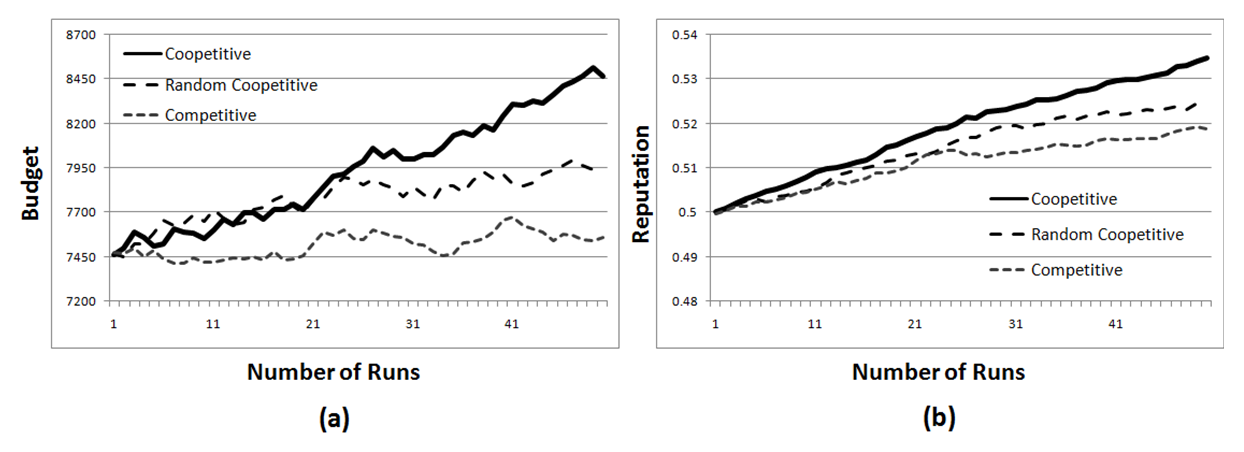
\includegraphics[scale=0.6]{graph1Final+.eps}
        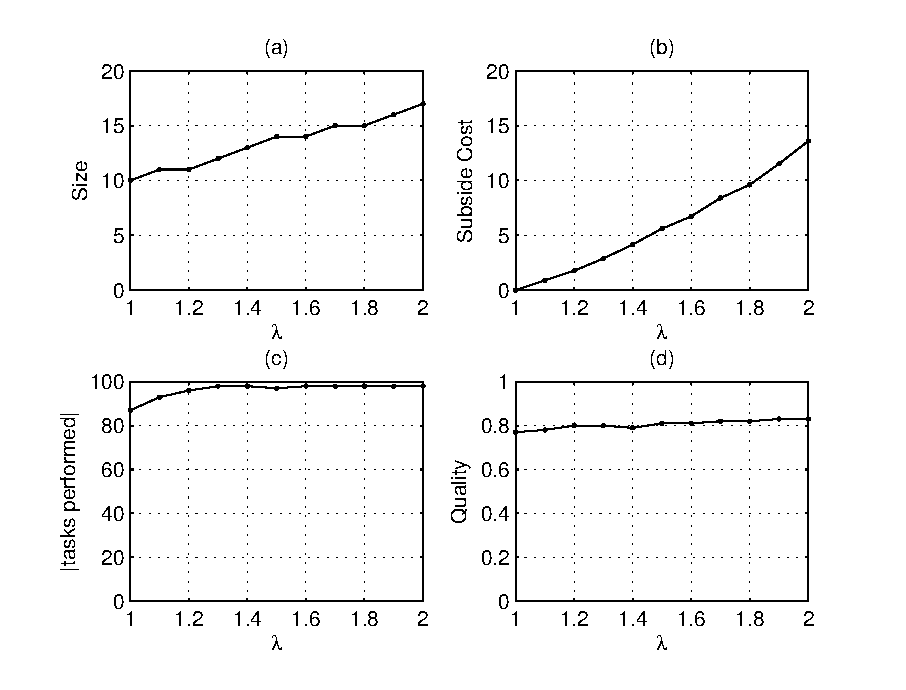
\includegraphics[width=3in]{figures/taxtation.eps}
        \caption{Analysis of community subsiding coefficient $\lambda$ on
        average community size (a), cost (b), number of tasks performed
        (c), and average quality of service of tasks performed (d).}
        \label{f_taxtation}
    \end{figure}
\end{frame}
%%%%%%%%%%%%%%%%%%%%%%%%%%%%%%%%%%%%%%%%%%%%%%%%%%%%%%%%%%%%%%%%%%%%%%%%%%%%%%

%%%%%%%%%%%%%%%%%%%%%%%%%%%%%%%%%%%%%%%%%%%%%%%%%%%%%%%%%%%%%%%%%%%%%%%%%%%%%%
\begin{frame}{Results: Taxation and Subsiding}
    \begin{figure}[!t]
        \centerline{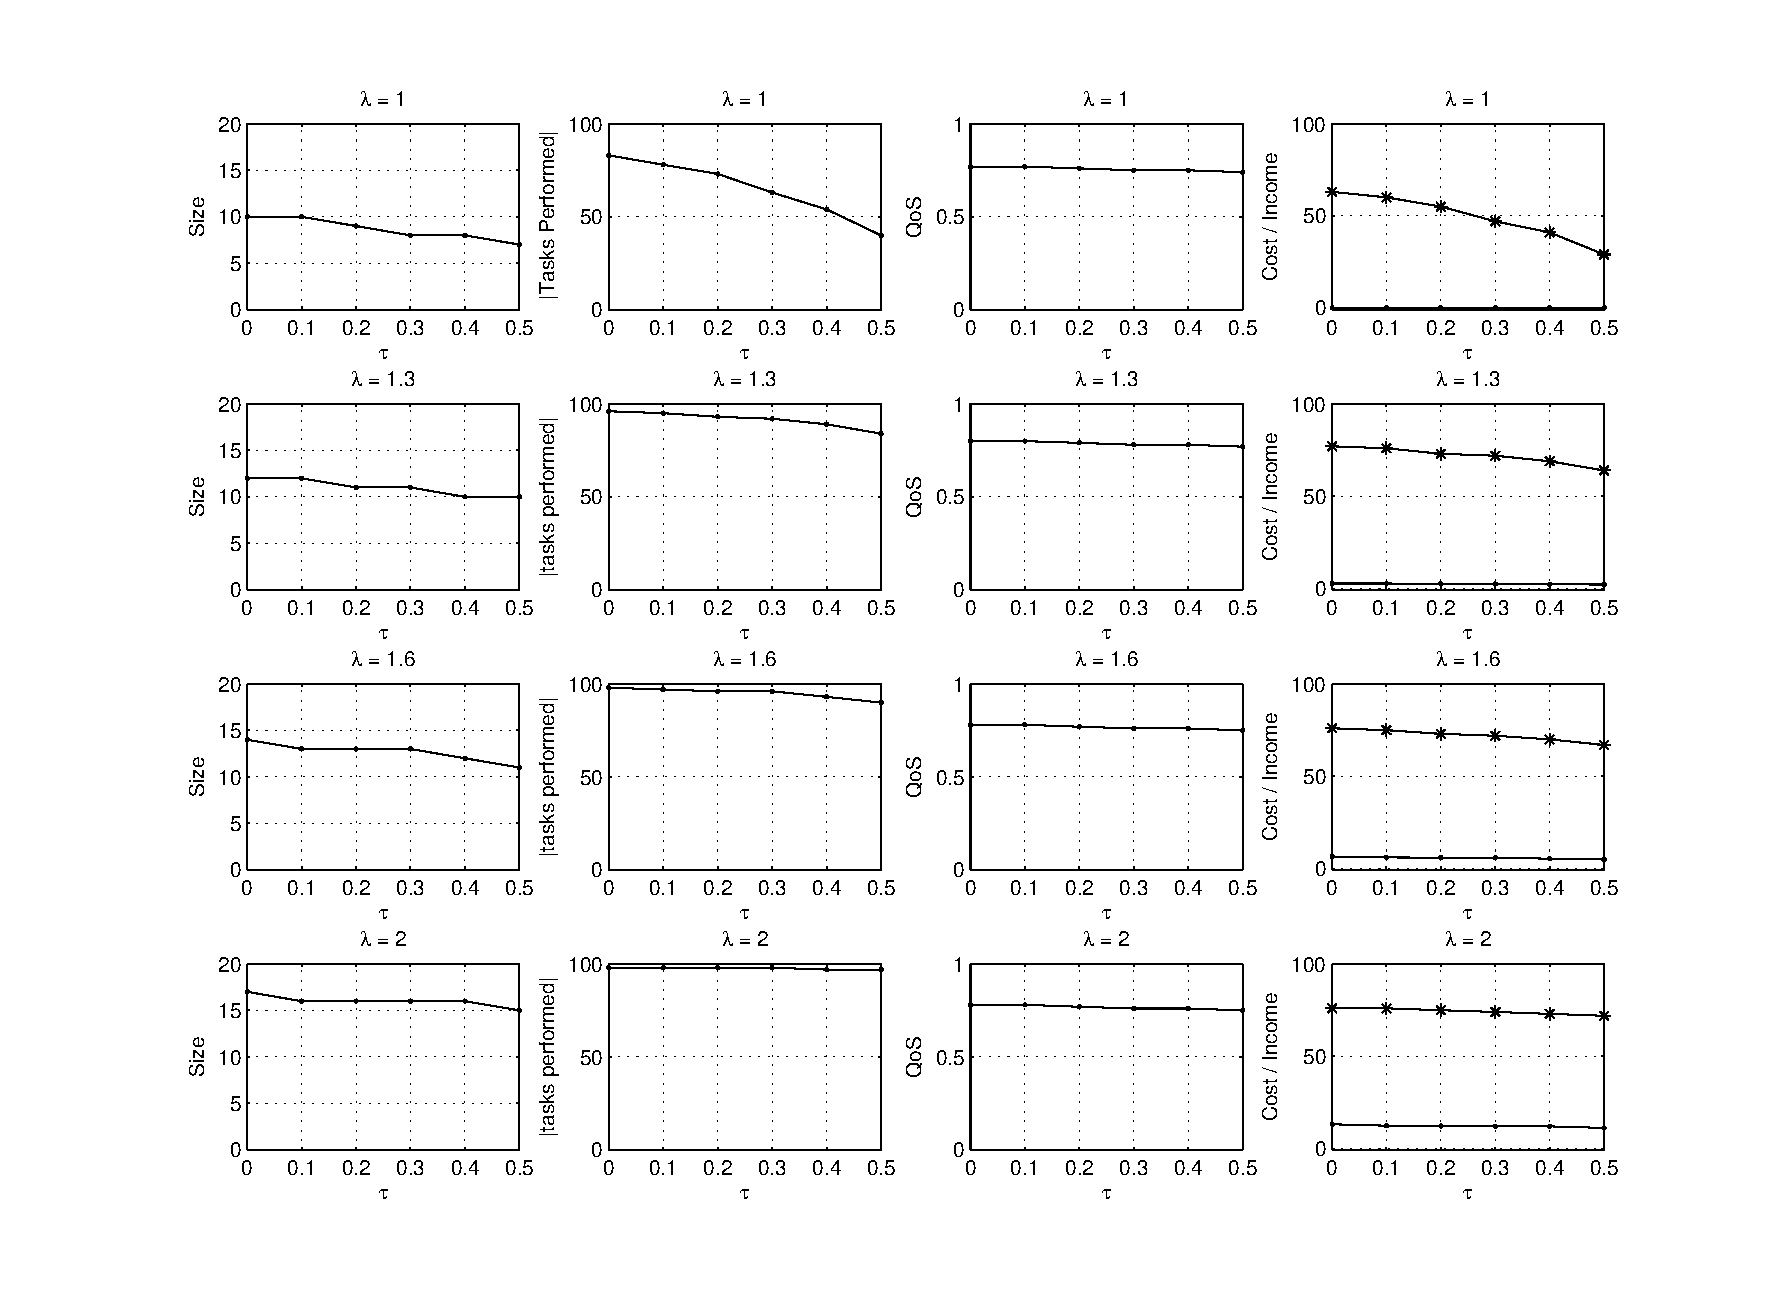
\includegraphics[width=4.2in]{figures/tax_dyn.eps}}
        \caption{Analysis of community subsiding coefficient $\lambda$
        having web service different stability levels of $\tau$ on average
        community size, number of tasks performed, average quality of
        service, and average cost/income of communities.}
        \label{fig_dynamic_taxtation}
    \end{figure}
\end{frame}
%%%%%%%%%%%%%%%%%%%%%%%%%%%%%%%%%%%%%%%%%%%%%%%%%%%%%%%%%%%%%%%%%%%%%%%%%%%%%%
%%%%%%%%%%%%%%%%%%%%%%%%%%%%%%%%%%%%%%%%%%%%%%%%%%%%%%%%%%%%%%%%%%%%%%%%%%%%%%%
\subsection{Representation and Complexity Issues}
\begin{frame}{Representation and Complexity Issues}
    \begin{itemize}
        \item Core and Shapley value are combinatorial problems.
        \item Input size is exponential.
        \item Compact or succinct representation of coalition games.
        \begin{itemize}
            \item A representation so that the input size is a polynomial in the number of agents.
        \end{itemize}
    \end{itemize}
\end{frame}
%%%%%%%%%%%%%%%%%%%%%%%%%%%%%%%%%%%%%%%%%%%%%%%%%%%%%%%%%%%%%%%%%%%%%%%%%%%%%%%

%%%%%%%%%%%%%%%%%%%%%%%%%%%%%%%%%%%%%%%%%%%%%%%%%%%%%%%%%%%%%%%%%%%%%%%%%%%%%%%
\begin{frame}{Different Compact Representations of Coalition Games}

    \begin{table}
        \small
        \begin{tabular}{l|c|c|c|c}
        Representations                  & Space    & Shapley                  & Core Existence  & Complete     \\ \hline
        Graph (w+)                       & P        & P                        & P               & Not          \\
        Graph                            & P        & NP-Complete              & NP-Complete     & Not          \\
        Synergy                          & NA       & P (l input)              & P               & Not          \\
        Multi-issue                      & NA       & P (l input)              & NP-Complete     & Complete     \\
        MC-net                           & NA       & P (l input)              & NP-hard         & Complete     \\
        Our method                       & P        & NP-hard                  & NP-hard         & Not          \\
        \end{tabular}
    \end{table}

    \begin{itemize}
        \item Our web service community valuation function representation ($v(C) = out(C)$) space requirement grows linearly to input size.
        \item As long as we keep our services aggregation valuation function v(C) linear, problem can be reduced to LP. Which Polynomial greedy and approximation algorithms already exists.
    \end{itemize}

\end{frame}


%%%%%%%%%%%%%%%%%%%%%%%%%%%%%%%%%%%%%%%%%%%%%%%%%%%%%%%%%%%%%%%%%%%%%%%%%%%%%%
\subsection{Distributed Decision Making for Dynamic Formation of Web Services Communites}
%%%%%%%%%%%%%%%%%%%%%%%%%%%%%%%%%%%%%%%%%%%%%%%%%%%%%%%%%%%%%%%%%%%%%%%%%%%%%%%
\begin{frame}{Distributed Decision Making for Dynamic Formation of Web Services Communites}
    \begin{figure}[htbp]
        \centering
        %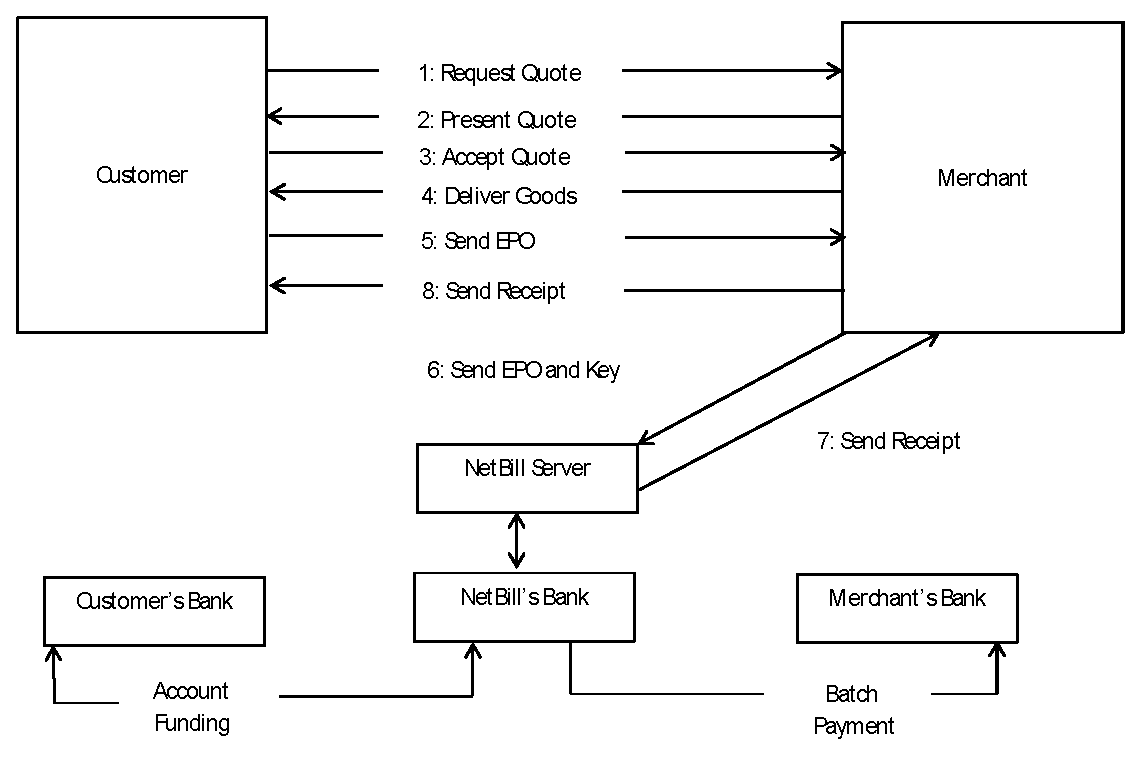
\includegraphics[width=12cm, height=8cm]{figures/figure1.eps}
        \includegraphics[width=0.9 \columnwidth]{figures/model_c2.eps}
        %%\includegraphics[scale=0.5]{figure1}
        %\caption{The NetBill payment protocol} \label{figure7}
    \end{figure}
\end{frame}

%%%%%%%%%%%%%%%%%%%%%%%%%%%%%%%%%%%%%%%%%%%%%%%%%%%%%%%%%%%%%%%%%%%%%%%%%%%%%%%
\begin{frame}{DDM: Distributed Decision Making Model}
    \begin{itemize}
        \item The architecture of centralized manager where most of the decisions are made by the centralized community manager, has practical problems in real world implementations.
        \item Web services and communities do not have complete information on all the details about other web services and communities in real world scenarios.
        \item We want to equip communities and web services with a decision making mechanism which would provide them with viable strategies and an estimation on long-term utility gain of choosing that strategy.
    \end{itemize}
\end{frame}
%%%%%%%%%%%%%%%%%%%%%%%%%%%%%%%%%%%%%%%%%%%%%%%%%%%%%%%%%%%%%%%%%%%%%%%%%%%%%%
\begin{frame}{DDM: Distributed Decision Making Model}
    \begin{figure}[htbp]
        \centering
        \includegraphics[width=0.9 \columnwidth]{figures/steps.eps}
    \end{figure}
\end{frame}



%%%%%%%%%%%%%%%%%%%%%%%%%%%%%%%%%%%%%%%%%%%%%%%%%%%%%%%%%%%%%%%%%%%%%%%%%%%%%%
\begin{frame}{DDM: Features}
    \begin{itemize}
        \item Features:
        \begin{itemize}
            \item $Th_{C} = \sum_{w \in C}{(Th_{w})}$ \textbf{(Throughput)}
            \item $A_{C} = 1-\prod_{w \in C}{(1-A_{w})}$ \textbf{(Availability)}
            \item $Et_{C} = max_{w \in C}{(Et_{w})}$ \textbf{(Execution Time)}
            \item $Exp1_i = Et_{i} - Et_{min}$ \textbf{(External Parameter 1)}
            \item $Exp2_i = Th_{max} - Th_{i}$ \textbf{(External Parameter 2)}
        \end{itemize}
        \item Utility:
        \begin{itemize}
            \item $U_{C} = f(A_{C}, Et_{C}, Exp1_{C}, Exp2_{C}, Th_{C})$
            \item $U_{C} = \big((\alpha \times (A_{C} - Et_{C}) - \beta \times (exp1_{C} + exp2_{C})\big) \times Th_{C}$
        \end{itemize}
    \end{itemize}
\end{frame}

%%%%%%%%%%%%%%%%%%%%%%%%%%%%%%%%%%%%%%%%%%%%%%%%%%%%%%%%%%%%%%%%%%%%%%%%%%%%%%
\begin{frame}{DDM: Feature Vectors}

    \begin{figure}[htbp]
        \centering
        \includegraphics[width=0.35 \columnwidth]{figures/cfvs.eps}
    \end{figure}

    \footnotesize
    \begin{itemize}
        \item \emph{Community Feature Vector:} $CFV_{<C>} = [f_1,...f_5]$
        \item \emph{Community Feature Vector Set:} $CFVS = \{CFV_{<C_1>}, \dots, CFV_{<C_N>}\}$
    \end{itemize}
\end{frame}




%%%%%%%%%%%%%%%%%%%%%%%%%%%%%%%%%%%%%%%%%%%%%%%%%%%%%%%%%%%%%%%%%%%%%%%%%%%%%%
\begin{frame}{DDM: Distributed Decision Making Model}
    \begin{table}[ht]
        \tiny
        \caption{An example of $gain$ matrix for 3 different communities and their combinations} % title of Table
        \centering % used for centering table
        {\renewcommand{\arraystretch}{1.2}
        \begin{tabular}{c|c c c c c c} % centered columns (4 columns)
        \hline\hline %inserts double horizontal lines
         & \textless348\textgreater & \textless1934\textgreater & \textless2117\textgreater & \textless348,194\textgreater & \textless194,217\textgreater & \textless348,194,217\textgreater \\ [0.5ex] % inserts table
        %heading
        \hline % inserts single horizontal line
        \textless348\textgreater & - & 0.282708 & 1.027081 & 0.282708 & 18.027081 & 18.027081 \\
        \textless194\textgreater & -2.637483 & - & 6.969072 & -2.637483 & 5.509583 & 4.387725 \\
        \textless217\textgreater & 5.027081 & 2.969072 & - & 5.509583 & 2.969072 & 5.509583 \\
        \textless348,1934\textgreater & 0.0 & 0.0 & -3.851432 & - & -3.851432 & -3.851432 \\
        \textless194,217\textgreater & 2.969072 & 0.0 & 0.0 & 2.969072 & - & 2.969072 \\
        \textless348,1934,217\textgreater & 0.0 & 0.0 & 0.0 & 0.0 & 0.0 & - \\ [1ex] % [1ex] adds vertical space
        \hline %inserts single line
        \end{tabular}
        }
        \label{table:nonlin} % is used to refer this table in the text
    \end{table}
        
    \footnotesize
    \begin{itemize}
        \item \emph{Ordered preference relation:} $C_1 \geq_{i}^t C_2 \geq_{i}^t ~\dots~ C_{i-1} \geq_{i}^t C_{i+1} \geq_{i}^t ~\dots~ C_n$    
    \end{itemize}
    
\end{frame}
%%%%%%%%%%%%%%%%%%%%%%%%%%%%%%%%%%%%%%%%%%%%%%%%%%%%%%%%%%%%%%%%%%%%%%%%%%%%%%
\begin{frame}{DDM: Distributed Decision Making Model}
    \footnotesize
    \begin{itemize}       
        \item {\color{blue}$K^t(C_i, k)$:} A set of $k$ most preferred communities of $C_i$ at time $t$:
            \footnotesize
            \begin{equation*}\label{h_t_pref_top}
                \begin{split}				
                    K^t(C_i, 0) = &\emptyset \\
                    K^t(C_i, k) = &\Big\{C_x | C_x \geq_{i}^t C_y ~\forall C_y \in CS ~\wedge~ C_x \neq C_y ~\wedge~ C_y \notin K^t(C_i, k-1) \Big\}				
                \end{split}
            \end{equation*}            
        \item {\color{blue}$L^t(C_i,k)$:} Both-sided preference. A set of $k$ most preferred communities of $C_i$ at time $t$ which they also have $C_i$ as their most $k$ preferred communities.
            \footnotesize
            \begin{equation*}\label{l_t_top_both}                
                L^t(C_i,k) = \Big\{C_j | C_j \in K^t(C_i, k)~ \wedge~ C_i \in K^t(C_j, k)\Big\}                 
            \end{equation*}
    \end{itemize}
\end{frame}
%%%%%%%%%%%%%%%%%%%%%%%%%%%%%%%%%%%%%%%%%%%%%%%%%%%%%%%%%%%%%%%%%%%%%%%%%%%%%%
\begin{frame}{DDM: Distributed Decision Making Model}
    \begin{figure}[htbp]
        \centering
        \includegraphics[scale=0.3]{figures/alg.png}
    \end{figure}
\end{frame}



\begin{frame}{DDM: Excremental Results}
    \begin{figure}[htbp]
    \centering
    \includegraphics[width=3in]{figures/utility_gain.eps}
    \caption{DDM against Rational: utility gain }
    \label{utility_gain_mlisa_and_rational}
    \end{figure}
\end{frame}
%%%%%%%%%%%%%%%%%%%%%%%%%%%%%%%%%%%%%%%%%%%%%%%%%%%%%%%%%%%%%%%%%%%%%%%%%%%%%%
\begin{frame}{DDM: Excremental Results}
    \begin{figure}[htbp]
        \centering
        \includegraphics[width=0.9 \columnwidth]{figures/roc.eps}
        %%\includegraphics[scale=0.5]{figure1}
        %\caption{The NetBill payment protocol} \label{figure7}
    \end{figure}
\end{frame}
%%%%%%%%%%%%%%%%%%%%%%%%%%%%%%%%%%%%%%%%%%%%%%%%%%%%%%%%%%%%%%%%%%%%%%%%%%%%%%
\begin{frame}{DDM: Excremental Results}
    \begin{table}[ht]
        \caption{Number of communities that misses the optimal decision, out of 1,000 communities} % title of Table
        \centering % used for centering table
        \begin{tabular}{|c|c|} % centered columns (4 columns)
        \hline %inserts double horizontal lines
         Method&Miss \\ [0.5ex] % inserts table
        %heading
        \hline % inserts single horizontal line
         DDM r=0.05& 375 \\ % inserting body of the table
         DDM r=0.07& 137 \\
         DDM r=0.10& 6 \\
         DDM r=0.20& 6 \\
        Rational Method& 717 \\
        Greedy Method& 828 \\ [1ex] % [1ex] adds vertical space
        \hline %inserts single line
        \end{tabular}
        \label{fail_rate} % is used to refer this table in the text
    \end{table}
\end{frame}
%%%%%%%%%%%%%%%%%%%%%%%%%%%%%%%%%%%%%%%%%%%%%%%%%%%%%%%%%%%%%%%%%%%%%%%%%%%%%%

%%%%%%%%%%%%%%%%%%%%%%%%%%%%%%%%%%%%%%%%%%%%%%%%%%%%%%%%%%%%%%%%%%%%%%%%%%%%%%
\subsection{Coopetitive Behavior of Services within Communities}
%%%%%%%%%%%%%%%%%%%%%%%%%%%%%%%%%%%%%%%%%%%%%%%%%%%%%%%%%%%%%%%%%%%%%%%%%%%%%%%
\begin{frame}{Coopetitive Behavior of Services within Communities}
    \begin{figure}[htbp]
        \centering
        %\includegraphics[width=12cm, height=8cm]{figures/figure1.eps}
        \includegraphics[width=0.9 \columnwidth]{figures/model_c3.eps}
        %%\includegraphics[scale=0.5]{figure1}
        %\caption{The NetBill payment protocol} \label{figure7}
    \end{figure}
\end{frame}
%%%%%%%%%%%%%%%%%%%%%%%%%%%%%%%%%%%%%%%%%%%%%%%%%%%%%%%%%%%%%%%%%%%%%%%%%%%%%%%

\begin{frame}{Coopetitive Behavior of Services within Communities}
    \begin{itemize}
        \item Within communities, services, selfish and utility maximizers by nature, can follow two different strategies, namely cooperation and competition in order to increase their payoffs when they provide services to consumers.
        \item To Model a competitive environment between autonomous services with different capabilities over tasks with different requirements.
        \item System Parameters:
        \begin{itemize}
            \item \textbf{Task QoS} ($T_{QoS}^r$)
            \item \textbf{Service QoS} ($QoS_w^r$)
            \item \textbf{Budget} ($B_w^t$)
            \item \textbf{Reputation} ($Rep_w^t$)
            \item \textbf{Growth Factor} ($G_w^t$)
        \end{itemize}
    \end{itemize}
\end{frame}
%%%%%%%%%%%%%%%%%%%%%%%%%%%%%%%%%%%%%%%%%%%%%%%%%%%%%%%%%%%%%%%%%%%%%%%%%%%%%%%



%%%%%%%%%%%%%%%%%%%%%%%%%%%%%%%%%%%%%%%%%%%%%%%%%%%%%%%%%%%%%%%%%%%%%%%%%%%%%%
\begin{frame}{Coopetitive Behavior of Services within Communities}
    \begin{figure}[h]
        \centering
        \includegraphics[scale=0.6]{figures/architecture++.eps}
%        \caption{Services are partitioned into competitive and cooperative
%        sets. Competitive services may get tasks directly from the master
%        agent and they can share it with other cooperative services in
%        their collaborative networks within the same community.}
        \label{architectureFigure}
    \end{figure}

    \begin{equation*} \label{repr}
        reward_w^r = \begin{cases}
        \eta + \upsilon \frac{QoS_w^r}{T_{QoS}^r+QoS_w^r}   & \text{if $T_{QoS}^r\leq QoS_w^r$;}\\
        -(\rho +  \upsilon \frac{T_{QoS}^r}{T_{QoS}^r+QoS_w^r} ) & \text{otherwise.}\\
        \end{cases}
    \end{equation*}


%    \begin{equation} \label{reward}
%        reward_w^t =
%        \begin{cases}
%        \frac{\sum_{r \in
%        task_w^t}reward_w^r}{|task_w^t|}& \text{if $task_w^t \neq \emptyset$;}\\
%        0 & \text{otherwise.}\\
%        \end{cases}
%    \end{equation}

%    \begin{equation*}\label{repz}
%        %Rep_{w}^{t+1} = Rep_{w}^{t} + reward
%        %\end{equation}
%        %\begin{equation*}
%        Rep_{w}^{t+1} = \begin{cases}
%
%        \Gamma & \text{if $ 0 \leq \Gamma \leq 1$;}\\
%        0  & \text{if $\Gamma < 0$;}\\
%        1 & \text{if $\Gamma > 1$.}\\
%        \end{cases}
%    \end{equation*}

    \begin{equation*}\label{eq:repreprowthfactor}
        Rep_{w}^{t+1} = (\alpha).Rep_{w}^{t} + (1-\alpha).reward_{w}^{t}
    \end{equation*}

    \begin{equation*}\label{eq:growthfactor}
        G^t_w = \frac{Rep^t_w + QoS_w^t+\frac{B_w^t}{n_t  \mu_w -
        \epsilon}}{3}
    \end{equation*}
%   \begin{equation*}
%        %\mu_{w} \in\{\mu_{w, CM}, \mu_{w, CO}\},~~~
%        QoS_w^t =
%        \begin{cases} \frac{\sum_{r \in
%        task_w^t}QoS_w^r}{|task_w^t|}& \text{if $task_w^t \neq \emptyset$;}\\
%        0 & \text{otherwise.}\\
%        \end{cases}
%    \end{equation*}

\end{frame}
%%%%%%%%%%%%%%%%%%%%%%%%%%%%%%%%%%%%%%%%%%%%%%%%%%%%%%%%%%%%%%%%%%%%%%%%%%%%%%%


%%%%%%%%%%%%%%%%%%%%%%%%%%%%%%%%%%%%%%%%%%%%%%%%%%%%%%%%%%%%%%%%%%%%%%%%%%%%%%
\begin{frame}{Experimental Results: Coopetitive}
    \begin{figure}%[h]
        %\centering
        %\includegraphics[scale=0.6]{graph1Final+.eps}
        \includegraphics[width=2.1in]{figures/graphbgtmed.eps}
        \includegraphics[width=2.1in]{figures/graphrep.eps}
        \caption{Part (a): Cumulative community budget comparison. Part
        (b): Average community reputation comparison over different
        strategic decisions.} \label{Graph1}
    \end{figure}
\end{frame}
%%%%%%%%%%%%%%%%%%%%%%%%%%%%%%%%%%%%%%%%%%%%%%%%%%%%%%%%%%%%%%%%%%%%%%%%%%%%%%


%%%%%%%%%%%%%%%%%%%%%%%%%%%%%%%%%%%%%%%%%%%%%%%%%%%%%%%%%%%%%%%%%%%%%%%%%%%%%%
\begin{frame}{Experimental Results: Coopetitive}
    \begin{figure}[h]
        \centering
        \includegraphics[width=1.45in]{figures/graphtaskdone.eps}
        \includegraphics[width=1.45in]{figures/graphtasksatisfaction.eps}
        \includegraphics[width=1.45in]{figures/graphavgqostask.eps}
        \caption{Overall performance from community's point of view. Part
        (a) Total number of tasks successfully done. Part (b) Ratio of
        tasks satisfied with required QoS. Part (c) Average QoS of
        performed tasks.} \label{graph_task}
    \end{figure}
\end{frame}
%%%%%%%%%%%%%%%%%%%%%%%%%%%%%%%%%%%%%%%%%%%%%%%%%%%%%%%%%%%%%%%%%%%%%%%%%%%%%%

%%%%%%%%%%%%%%%%%%%%%%%%%%%%%%%%%%%%%%%%%%%%%%%%%%%%%%%%%%%%%%%%%%%%%%%%%%%%%%%
%\begin{frame}{Reinforcement Learning: Q-learning - (Phase 3)}
%    \begin{itemize}
%        \item MDP (Markov Game):
%        \begin{itemize}
%            \item \emph{S}: Set of states
%            \item \emph{A}: Actions
%            \item \emph{$T: S \times A_1 \times A_2 \times ... \times A_k \rightarrow P(s) $}
%            \item \emph{$R: S \times A_1 \times A_2 \times ... \times A_k \rightarrow Reward(s,a) $}
%        \end{itemize}
%    \end{itemize}
%
%    \begin{itemize}
%        \item Q-Learning, the goal is to learn:
%        \begin{itemize}
%            \item The probability of others playing actions from action set on each state.
%            \item $V(s): $ Expected reward over time, starting from state $s$
%            \item $Q(s,a,o): $ Expected reward taking action $a$ when other players chose action $a$ from state $s$
%        \end{itemize}
%    \end{itemize}
%
%    \begin{equation*}
%        {\color{blue}V(s)} = max min \sum_{a \in A}{{\color{green}Q(s,a,o)} \times T(s,a,s')}
%    \end{equation*}
%
%    \begin{equation*}
%        {\color{green}Q(s,a,o)} = R(s,a,o) + \gamma\sum{s'}{T(s,a,o,s'){\color{blue}V(s')}}
%    \end{equation*}
%
%\end{frame}
%%%%%%%%%%%%%%%%%%%%%%%%%%%%%%%%%%%%%%%%%%%%%%%%%%%%%%%%%%%%%%%%%%%%%%%%%%%%%%%%
%
%%%%%%%%%%%%%%%%%%%%%%%%%%%%%%%%%%%%%%%%%%%%%%%%%%%%%%%%%%%%%%%%%%%%%%%%%%%%%%%
%\begin{frame}{Prilimanary Results: Q-learning - (Phase 3)}
%    \begin{table}[!htb]
%        %\caption{Global caption}
%        \begin{minipage}{.5\linewidth}
%          \caption{Q1}
%          \centering
%            \begin{tabular}{ r|c|c| }
%                \multicolumn{1}{r}{}
%                 &  \multicolumn{1}{c}{Comp}
%                 & \multicolumn{1}{c}{Coop} \\
%                \cline{2-3}
%                Comp & 2.434 & 2.624 \\
%                \cline{2-3}
%                Coop & -0.269 & -0.136 \\
%                \cline{2-3}
%            \end{tabular}
%        \end{minipage}%
%        \begin{minipage}{.5\linewidth}
%          \centering
%            \caption{Q2}
%            \begin{tabular}{ r|c|c| }
%                \multicolumn{1}{r}{}
%                 &  \multicolumn{1}{c}{Comp}
%                 & \multicolumn{1}{c}{Coop} \\
%                \cline{2-3}
%                Comp & 0.897 & -0.126 \\
%                \cline{2-3}
%                Coop & 1.084 & 0.4 \\
%                \cline{2-3}
%            \end{tabular}
%        \end{minipage}
%    \end{table}
%
%    \begin{table}[!htb]
%        %\caption{Global caption}
%        \begin{minipage}{.5\linewidth}
%          \caption{Q3}
%          \centering
%            \begin{tabular}{ r|c|c| }
%                \multicolumn{1}{r}{}
%                 &  \multicolumn{1}{c}{Comp}
%                 & \multicolumn{1}{c}{Coop} \\
%                \cline{2-3}
%                Comp & 2.064 & 1.826 \\
%                \cline{2-3}
%                Coop & 0.564 & -0.364 \\
%                \cline{2-3}
%            \end{tabular}
%        \end{minipage}%
%        \begin{minipage}{.5\linewidth}
%          \centering
%            \caption{Q4}
%            \begin{tabular}{ r|c|c| }
%                \multicolumn{1}{r}{}
%                 &  \multicolumn{1}{c}{Comp}
%                 & \multicolumn{1}{c}{Coop} \\
%                \cline{2-3}
%                Comp & -0.261 & -0.436 \\
%                \cline{2-3}
%                Coop & 0.725 & 0.632 \\
%                \cline{2-3}
%            \end{tabular}
%        \end{minipage}
%    \end{table}
%
%\end{frame}
%%%%%%%%%%%%%%%%%%%%%%%%%%%%%%%%%%%%%%%%%%%%%%%%%%%%%%%%%%%%%%%%%%%%%%%%%%%%%%%

%%%%%%%%%%%%%%%%%%%%%%%%%%%%%%%%


%\begin{frame}{Results: Coalition Formation}
%    \begin{figure}[!t]
%        \centering
%        %\includegraphics[scale=0.6]{graph1Final+.eps}
%        \includegraphics[width=3in]{figures/least_core.eps}
%        \caption{Analysis of \emph{$\epsilon$-core} set non-emptiness, for different values of $\epsilon$}. \label{f_leastcore}
%    \end{figure}
%\end{frame}
%%%%%%%%%%%%%%%%%%%%%%%%%%%%%%%%%%%%%%%%%%%%%%%%%%%%%%%%%%%%%%%%%%%%%%%%%%%%%%

%%%%%%%%%%%%%%%%%%%%%%%%%%%%%%%%%%%%%%%%%%%%%%%%%%%%%%%%%%%%%%%%%%%%%%%%%%%%%%%
%\begin{frame}{Results: Coalition Formation}
%    \begin{figure}[!t]
%        \centering
%        %\includegraphics[scale=0.6]{graph1Final+.eps}
%        \includegraphics[width=2.1in]{figures/s2_task_done.eps}
%        \includegraphics[width=2.1in]{figures/s2_task_qos.eps}
%        \caption{Part (a): Cumulative number of tasks successfully performed. Part
%        (b): Average QoS of tasks performed.} \label{performancemany}
%    \end{figure}
%\end{frame}
%
%%%%%%%%%%%%%%%%%%%%%%%%%%%%%%%%%%%%%%%%%%%%%%%%%%%%%%%%%%%%%%%%%%%%%%%%%%%%%%%
%\begin{frame}{Results: Coalition Formation}
%    \begin{figure}[!t]
%        \centering
%        %\includegraphics[scale=0.6]{graph1Final+.eps}
%        \includegraphics[width=1.45in]{figures/avg_task_ws_done.eps}
%        \includegraphics[width=1.45in]{figures/avg_qos_ws_done.eps}
%        \includegraphics[width=1.45in]{figures/avg_avail_ws_done.eps}
%        \caption{A comparison between our community model and the high availability community model, on communities of size 4,5,6 only. Part (a): Cumulative number of tasks successfully performed. Part
%        (b): Average QoS of tasks performed. (c) Average Community Service Availability} \label{fig_avail_method}
%    \end{figure}
%\end{frame}
%%%%%%%%%%%%%%%%%%%%%%%%%%%%%%%%%%%%%%%%%%%%%%%%%%%%%%%%%%%%%%%%%%%%%%%%%%%%%%%






%\begin{frame}{Results: Coopetitive}
%    \begin{figure}[h]
%        \centering
%        \includegraphics[scale=1.45in]{figures/graphbgtmed3set.eps}
%        \includegraphics[scale=1.45in]{figures/graphbgthigh.eps}
%        \includegraphics[scale=1.45in]{figures/graphbgtveryhigh.eps}
%        \caption{High membership fees or less task income impacts on
%        different selection strategies. Part (a) Medium membership fee.
%        Part (b) High membership fee. Part (c) Very high membership fee.}
%        \label{membership_fee_graph}
%    \end{figure}
%\end{frame}


%%%%%%%%%%%%%%%%%%%%%%%%%%%%%%%% frame30 outline page
%%%%%%%%%%%%%%%%%%%%%%%%%%%%%%%%%%%%%%%%%%%%%%%%%%%%%%%%%%%%%%%%%%%%%%%%%%%%%%%
\section{Conclusion}
\begin{frame}{Conclusion and Feature Work}
    \begin{itemize}
     	\itemsep=.5cm
    	\item Introduction
    	\item Background and Literature Review
    	\item Proposed Research
    	\item {\bf Conclusion and Feature Work}
    \end{itemize}
\end{frame}

%%%%%%%%%%%%%%%%%%%%%%%%%%%%%%%%%%%%%%%%%%%%%%%%%%%%%%%%%%%%%%%%%%%%%%%%%%%%%%
\subsection{Conclusion}
\begin{frame}{Contributions}
    \begin{itemize}     	
        	\item An optimal method for formation and membership management of communities of web services ensuring satisfaction of all the members involved and stability of group.
        	\item Proposing a valuation function and an approximation algorithm for convexity check of coalitions, making decision making practical in real-time settings for our web service community settings.
        	\item Proposed a novel approach for training communities using a small set of training data, to be able to efficiently make decisions in distributed and real-world environments where information is not complete.
    \end{itemize}
\end{frame}

%%%%%%%%%%%%%%%%%%%%%%%%%%%%%%%%%%%%%%%%%%%%%%%%%%%%%%%%%%%%%%%%%%%%%%%%%%%%%%
\begin{frame}{Future Work}
    \begin{itemize}     	
    	\item Implement communities using bargaining theory where agents can have side payments to insure group stability
    	\item More analytical and theoretical analysis on the convexity condition and also minimal $\epsilon$ values in \emph{$\epsilon$-core} solution concepts and constant factor  of our $Depth-k$ approximation algorithm.
    	\item Using the SVM machine learning algorithm as learning algorithm for training our data set to better distinguish decisions based on long-term utility.
    \end{itemize}
\end{frame}


%%%%%%%%%%%%%%%%%%%%%%%%%%%%%%%%%%%%%%%%%%%%%%%%%%%%%%%%%%%%%%%%%%%%%%%%%%%%%%%
%%%%%%%%%%%%%%%%%%%%%%%%%%%%%%%%%%%%
%%%%%%%%%%%%%%%%%%%%%%%%%%%%%%%%%%%%%%%%%%%%%%%%%%%%%%%%%%%%%%%%%%%%%%%%%%%%%%
\begin{frame}{Publications}
    \scriptsize
    \begin{enumerate}
        \item Submitted a Journal Paper at Decision Support Systems; \emph{``Distributed Decision Making for Dynamic Formation of Web Services Communities.''}, July. 2015
        \item Published a Journal Paper at IEEE Transactions on Services Computing; \emph{``Efficient Community Formation for Web Services.''}, (Impact factor: 3.09), August. 2015
        \item Published a Journal Paper at the International Journal of Expert Systems With Applications; \emph{``To Compete or to Cooperate? This is the Question in Communities of Autonomous Services''},  (Impact factor: 1.854, 5-year: 2.339), Jan 2014
        \item Published a Paper in 10th IEEE International Conference on Services Computing; \emph{``Efficient Coalition Formation for Web Services''}, 2013
        \item Published a Paper in the 10th International Conference on Service Oriented Computing (ICSOC 2012); \emph{``Analyzing Coopetition Strategies of Services within Communities''}, 2012
    \end{enumerate}
\end{frame}

%%%%%%%%%%%%%%%%%%%%%%%%%%%%%%%%%%%%%%%%%%%%%%%%%%%%%%%%%%%%%%%%%%%%%%%%%%%%%%%%
%\begin{frame}{Induced Subgraph Games}
%    \begin{itemize}
%        \item An induced subgraph game is a coalitional game defined by an undirected weighted graph $G = (V,W)$ where $V$ is the set of vertices and $W : V \rightarrow V$ is the set of edges weights. For $(i,j) \in V^2$, $w_{ij}$ is the weight of the edge between $i$ and $j$.
%        \item $N = V$
%        \item for all $C \subseteq N, v(C) = \sum_{(i,j) \in C} w_{ij}$
%        \item {\color{blue}Space Complexity:} Using an adjacency matrix, we need to provide $n^2$ entries.
%        \item {\color{blue}Convexity:} If all the weights are nonnegative then the game is convex.
%        \item {\color{blue}Shapley Value:} $\phi_i(N,v) = \frac{1}{2} \sum_{(i,j) \in N^2 | i \neq j}w_{ij}$
%        \item This is {\color{blue}not complete}. Many coalition games cannot be represented by a induced subgraph game.
%
%    \end{itemize}
%\end{frame}


%%%%%%%%%%%%%%%%%%%%%%%%%%%%%%%%%%%%%%%%%%%%%%%%%%%%%%%%%%%%%%%%%%%%%%%%%%%%%%

\begin{frame}{Questions}
    \begin{figure}[!t]
    \centering
    %\includegraphics[scale=0.6]{graph1Final+.eps}
    \includegraphics[width=2.1in]{figures/question.eps}
    \label{questionfig}
    \end{figure}
\end{frame}
%%%%%%%%%%%%%%%%%%%%%%%%%%%%%%%%%%%%%%%%%%%%%%%%%%%%%%%%%%%%%%%%%%%%%%%%%%%%%%


\end{document}
